%%% code: 代码文件夹
%%% figures: 图片文件夹
%%% *.cls: LaTeX 格式文件
%%% *.tex: LaTeX 文档文件
%%% *.bib: Bib 引用文献源文件
\documentclass{mcmthesis}  % 文档类型
\mcmsetup{CTeX = false,   % 使用 CTeX 套装时，设置为 true
	tcn = 2602805,   % 队伍控制号
	problem = A,  % 选题
	sheet = true,   % sheet页
	titleinsheet = true,   % sheet页显示标题
	keywordsinsheet = true,  % sheet页显示关键词
	titlepage = false,   % 标题页
	abstract = true  % 摘要
}
%%%%%%%%%%%%%%%%%%%%%%%%%%%%%%%%%%%%%%%%%%%%%%%%%%%%%%%

%%%%%%%%%%%%%%%%%%%%%%%%%%%%%%%%%%%%%%%%%%%%%%%%%%%%%%%
%%% 导入宏包和引用文献源
%%%%%%%%%%%%%%%%%%%%%%%%%%%%%%%%%%%%%%%%%%%%%%%%%%%%%%%
\usepackage{pgfplots}
\pgfplotsset{compat=1.18}
%\usepackage{palatino}  % 帕拉提诺体字体宏包
\usepackage{times}  % 正文使用Times New Roman风格字体
\usepackage{newtxmath}
\usepackage{lipsum}  % 导入生成段落的宏包
\usepackage{indentfirst}
\usepackage{booktabs} % For professional-looking tables
\usepackage{xcolor}   % For cell coloring
\usepackage{colortbl} % Required for \rowcolor
\definecolor{LightGreen}{rgb}{0.9, 0.95, 0.9}
\definecolor{pink}{RGB}{229, 238, 255}
\usepackage{fancyhdr}
\usepackage{enumitem} % 用于自定义列表格式
\usepackage{setspace}
\usepackage{svg}
\usepackage{booktabs}  % 三线表加粗
\usepackage{float}
\usepackage{eso-pic}  % 用于在页面添加背景
\usepackage{graphicx} % 图片支持
\usepackage{tikz}     % 用于绘制半透明覆盖层
\usepackage{subcaption}
\usepackage{caption}
\setlist[itemize]{listparindent=2em}
\setlist[enumerate]{listparindent=2em}
\usepackage[titles]{tocloft}
\usepackage{tabularx}
\setlength{\cftbeforesecskip}{3pt}   % 节之前的间距
\setlength{\cftbeforesubsecskip}{1.5pt} % 小节之前的间距
\newcommand{\upcite}[1]{\textsuperscript{\textsuperscript{\cite{#1}}}}
\urlstyle{rm}
\usepackage{CTeX}
\setlength{\headheight}{13.6pt}
%%%%%%%%%%%%%%%%%%%%%%%%%%%%%%%%%%%%%%%%%%%%%%%%%%%%%%%

%%%%%%%%%%%%%%%%%%%%%%%%%%%%%%%%%%%%%%%%%%%%%%%%%%%%%%%
%%% 文档信息设置
%%%%%%%%%%%%%%%%%%%%%%%%%%%%%%%%%%%%%%%%%%%%%%%%%%%%%%%
\title{Beyond the Black Box: A Multifactor Differential Model for Smartphone Power Drain}  % 文章标题
\author{\small Team 2602805}  % 作者，开启标题页才会显示
\date{\today}  % 日期，开启标题页才会显示

%%%%%%%%%%%%%%%%%%%%%%%%%%%%%%%%%%%%%%%%%%%%%%%%%%%%%%%
%%% 文档开始
%%%%%%%%%%%%%%%%%%%%%%%%%%%%%%%%%%%%%%%%%%%%%%%%%%%%%%%
\begin{document}  % 文档
	\begin{abstract}  % 摘要
		
		在现代生活中，智能手机电池续航同时受到用户使用强度、处理器负载、环境温度等多因素的综合影响，并受锂离子电池充电历史与老化进程的制约。为此，本文构建了连续时间微分方程模型，以刻画电池电量的时间动态变化规律，实现对不同使用场景下剩余续航时间的准确预测。
		
		\textbf{首先}，我们建立了 SOC 动态微分方程的基础模型，从多维度考量总功率的构成，\textbf{明确各功率分量的特性}，并进一步纳入温度影响以改进模型。采用 \textbf{Runge–Kutta 方法}对微分方程进行数值求解。随机仿真结果表明，在 Wi‑Fi 网络环境下电池使用时间为 \textbf{10.66 小时}，与实际手机使用情况吻合，验证了所建模型的有效性。最后，我们说明了参数估计方法，进一步确认了模型的可靠性。
		
		\textbf{其次}，我们选取了若干典型使用场景进行“耗尽时间”预测。结果表明，\textbf{GPS、CPU 负载和屏幕亮度对电池寿命影响显著}，\textbf{其中 GPS 导致的电池寿命降幅最高达 40.354\%}。通过蒙特卡洛模拟对影响因素的不确定性进行分析，不同场景下的 \textbf{CV 值介于 2\% 至 4.5\% 之间}，表明模型具有较强的稳健性。最后，通过敏感性指标对模型表现进行评价。
		
		\textbf{接着}，我们验证了模型假设的合理性并分析了模型的敏感性。通过改变屏幕类型假设，验证了\textbf{模型对不同屏幕类型的广泛适应性}。基于热‑效率反馈机制的随机仿真结果表明，关键使用参数的敏感性排序保持不变，且\textbf{模型输出变化仅为 0.25\%}，证实了模型假设的有效性。利用 SRC、VIF 和 CV 值进行参数敏感性分析，得到 \textbf{CV 值仅为 5.52\%}，说明模型具有良好的稳定性与可靠性。最后，对\textbf{使用模式波动}进行分析，发现\textbf{当行为更新间隔设为 60 分钟时，电池寿命达到最大值 12.36 小时，相比最差状态提升 17.4\%}。
		
		\textbf{最后}，结合电池老化的影响，我们为用户和操作系统提出建议：\textbf{建议用户按需启用核心模块，并建议操作系统实施核心参数的精细管控等措施}。进一步将模型应用于智能手环，显示出其\textbf{在设备间的泛化能力}。
		\begin{keywords}
			微分方程、随机模拟、蒙特卡罗模拟、荷电状态 (SOC)、电池寿命
		\end{keywords}
	\end{abstract}  % 结束摘要
	\maketitle  % 生成sheet页
	
	\tableofcontents  % 生成目录表
	\setcounter{page}{2} % 重置页码为 2
	
	%%%%%%%%%%%%%%%%%% sheet页与目录页结束 %%%%%%%%%%%%%%%%%%
	
	\newpage  % 开始新的一页
	\section{Introduction}  % 一级标题
	\subsection{Background}  % 二级标题
	在现代社会中，智能手机已成为不可或缺的工具，然而其电池续航行为常呈现出难以预测的特性：有时可满足全天使用，有时则在午前便迅速耗尽。尽管部分用户将其归因于“重度使用”，但电池耗电的真正驱动因素远为复杂。实际功耗取决于屏幕尺寸与亮度、处理器负载、网络活动以及后台应用程序（即便设备处于空闲状态仍持续耗能）之间的动态交互。环境温度等因素进一步增加了问题的复杂性：部分电池在低温环境下有效容量下降，或在持续高负载下过热运行。此外，电池的性能也受其使用历史与充电习惯的影响。
	
	因此，建立能够准确描述智能手机电池行为的数学模型，成为预测续航表现、优化使用策略的重要基础。本研究聚焦于构建基于连续时间的锂离子电池电量动态模型，旨在表征实际使用场景下电池荷电状态随时间变化的函数关系，并用于预测不同条件下的剩余使用时间。该模型不仅应反映多因素耦合的耗电机制，还需兼顾电池老化等长期效应，从而为终端用户提供切实可行的电量管理建议，并为操作系统层面的节能策略设计提供理论依据。
	
	\begin{figure}[h!]
		\centering
		% trim = 左边裁剪 下边裁剪 右边裁剪 上边裁剪（单位：cm）
		% clip 表示启用裁剪功能
		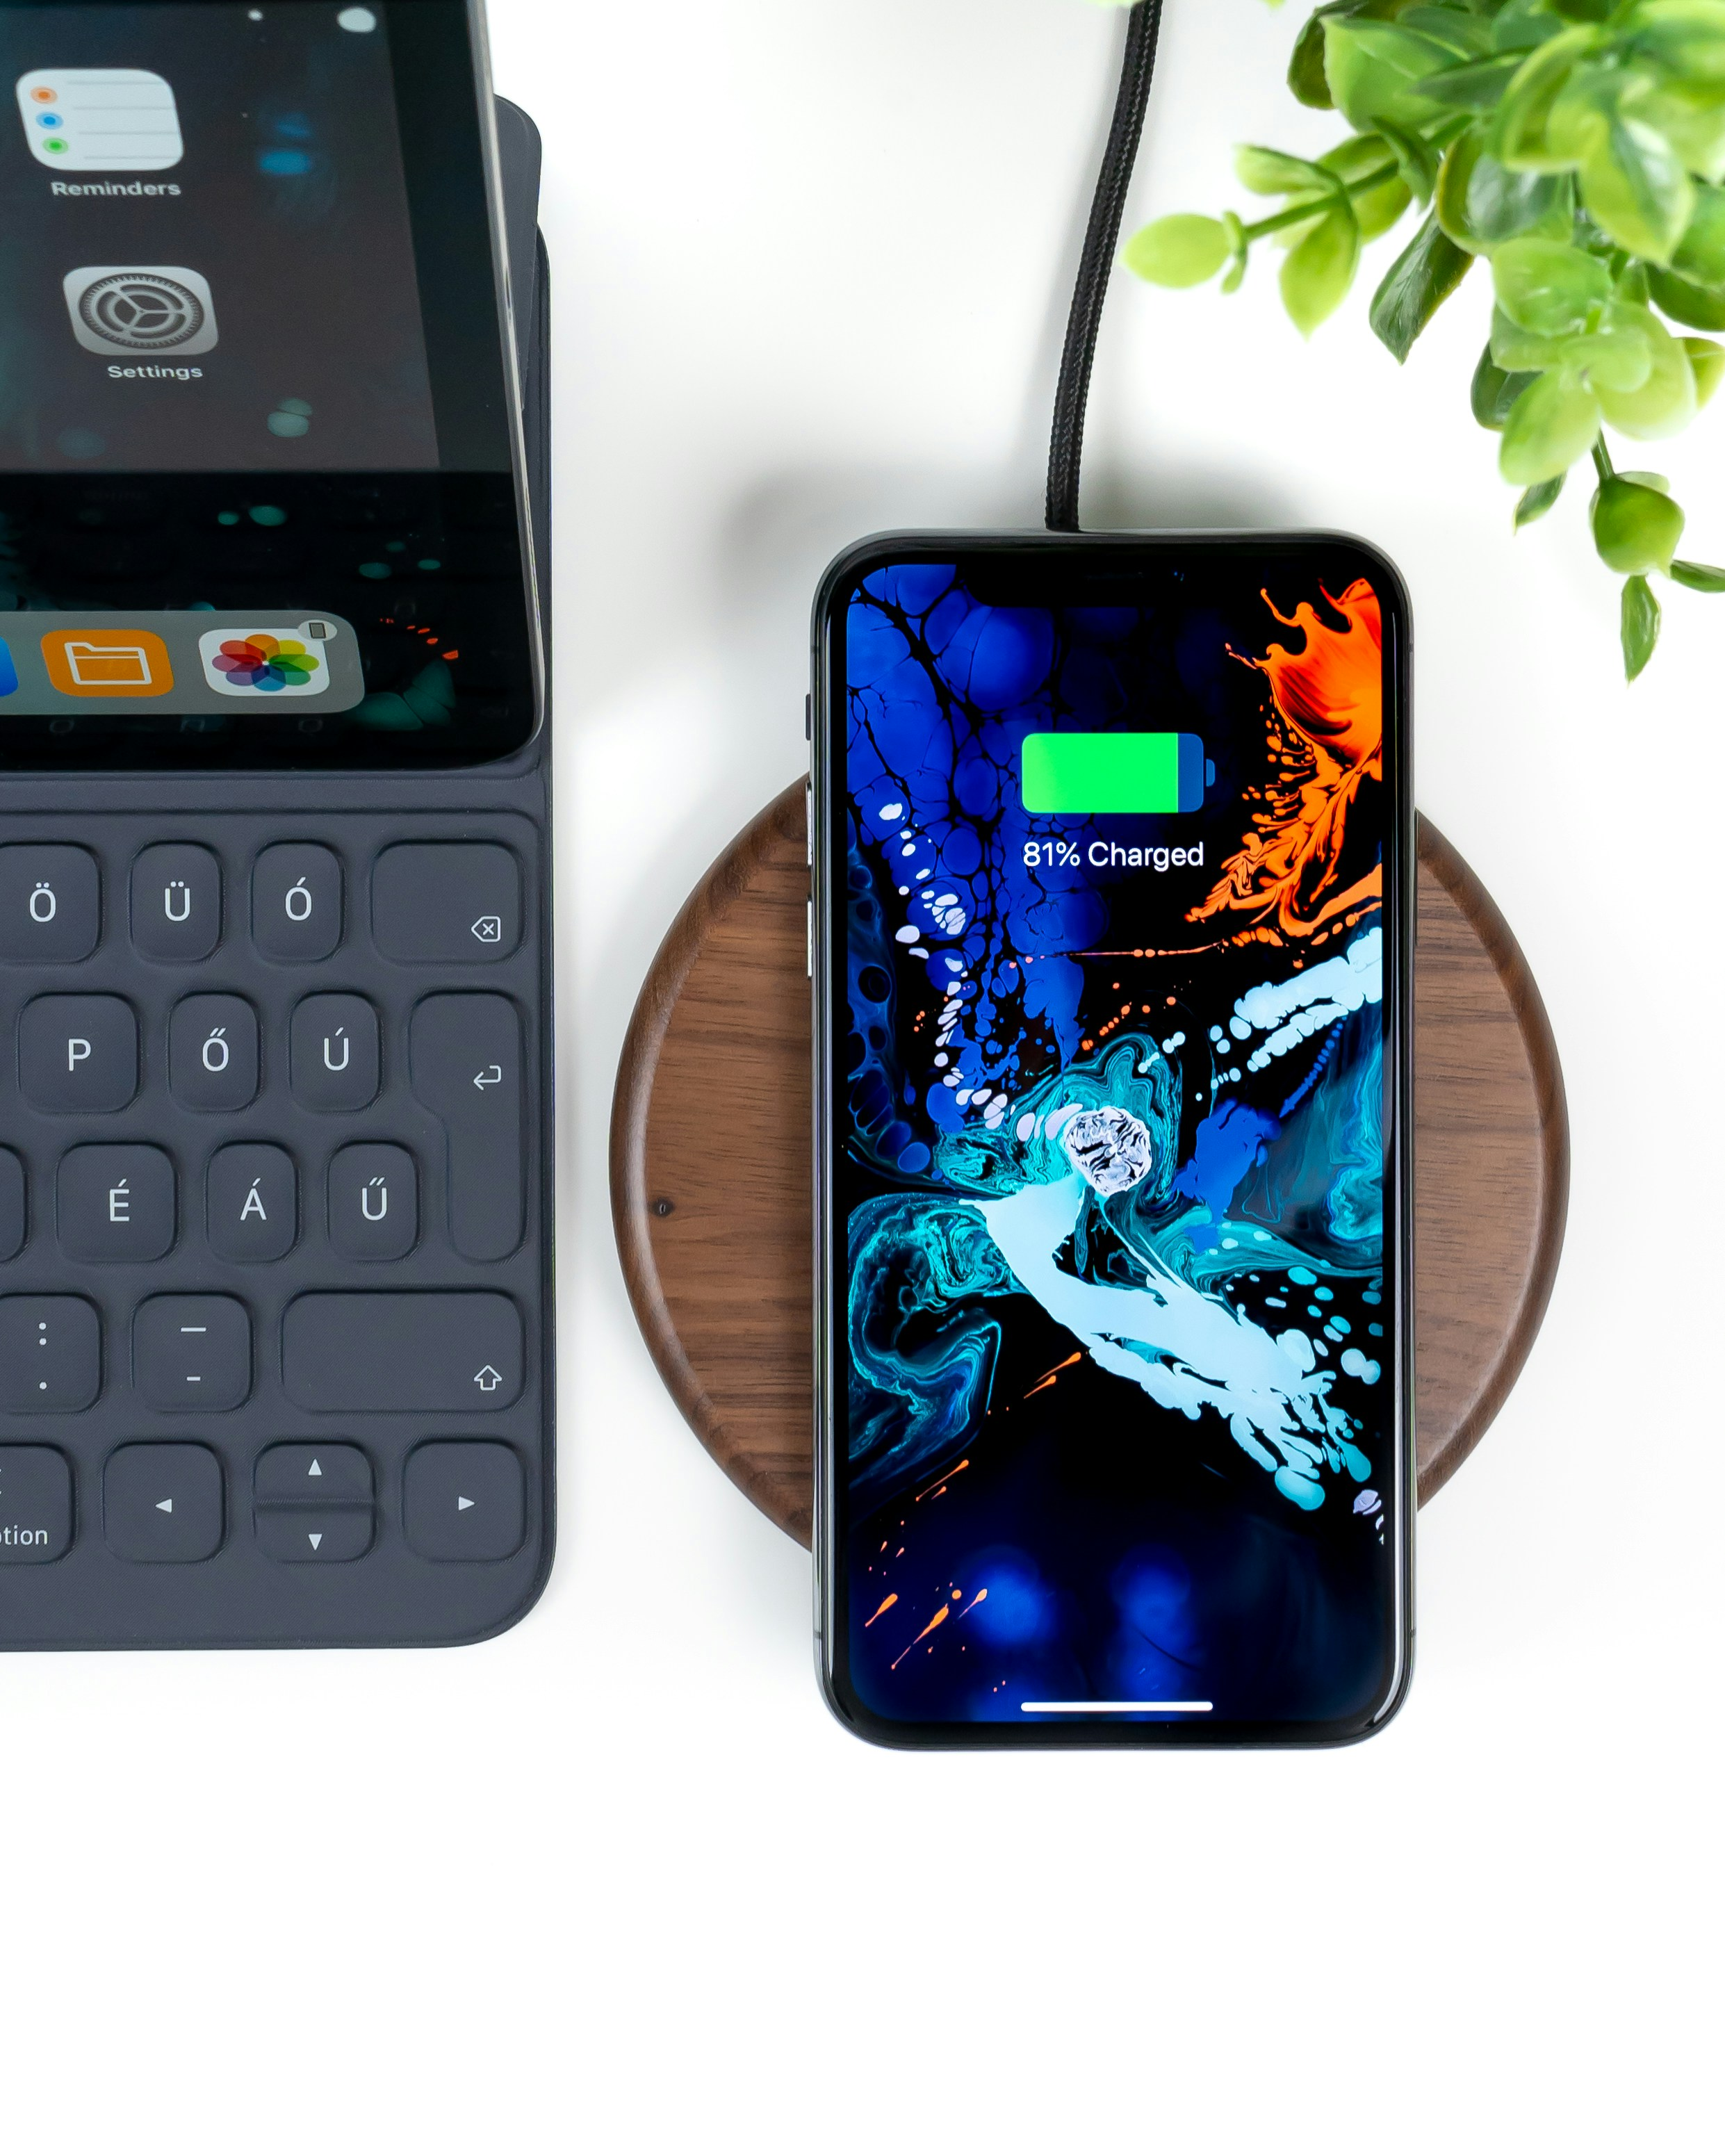
\includegraphics[
		width=0.5\textwidth,
		trim=0cm 15cm 0cm 0cm,  % 仅上方裁剪1厘米，其他边不裁剪
		clip
		]{figures/无线充电.jpg}
		\caption{无线充电}
	\end{figure}
	
	\subsection{Restatement of the Problem}
	根据问题描述中有关电池放电的相关条件和基本信息，以下问题需要解决：
	\begin{itemize}
		\item 构建一个综合考虑屏幕亮度、后台进程等多种因素的电池耗电连续时间模型。机器学习和时间序列不能满足需求。
		\item 利用该模型预测不同初始电量及使用状态下的剩余可用时间，分析不确定性结果的产生原因，并系统评估各类使用活动与环境条件对电池寿命及耗电速率的影响。
		\item 对模型进行灵敏度分析。研究在改变假设、参数值和使用模式波动后，模型预测结果的变化。
		\item 给手机使用者提供建议，缩短电池老化时间，降低电量消耗，延长手机使用时间 。并说明如何将该模型运用到其他便携式设备，比如笔记本电脑，智能手表上。
	\end{itemize}
	
	\subsection{Our Work \& Model Overview}
	\indent After analyzing the problem, our team searched for data and built three main models to solve it. To avoid a complicated description and clearly show our work process, the flow chart is presented in Figure \ref{fig:2026美赛流程图}.
	
	Considering the background, we analyze and solve the problems step-by-step:
	
	\textbf{Step 1}: \textbf{建立基础的电池电量动态微分方程模型。}
	
	\textbf{Step 2}: \textbf{扩展模型以纳入多因素影响。}纳入CPU负载、后台进程、网络状态、屏幕亮度、环境温度等因素，兼顾OLED与LCD屏幕类型的功耗差异及GPS工作状态等，构建微分方程，利用RK法求解。
	
	\textbf{Step 3}: \textbf{模型预测与结果分析。}利用模型预测不同初始电量与使用场景下的剩余电量，将预测结果与实际观测数据进行比较，分析预测差异的来源，系统评估各类使用活动与环境条件对电池耗电速率与寿命的影响。
	
	\textbf{Step 4}:\textbf{灵敏度分析与模型稳定性检验。} 通过调整模型假设、引进SRC,VIF,CV来探究关键参数、改变切换模式频率探究fluctuation of usage patterns，来研究预测结果的敏感性，评估模型在不同条件下的稳健性与可靠性。 
	
	\textbf{Step 5}: \textbf{用户建议与模型泛化应用。}基于建模结果，为用户提供可操作的电池使用建议，以延缓电池老化、降低能耗并延长续航时间。进一步探讨该模型在笔记本电脑、智能手表等其它便携设备中的适用性与推广潜力。
	
	For better arranging our process of problem solving, the flow diagram of our work is shown in Figure \ref{fig:2026美赛流程图}.
	
	\begin{figure}[h!]
		\centering
		% trim = 左边裁剪 下边裁剪 右边裁剪 上边裁剪（单位：cm）
		% clip 表示启用裁剪功能
		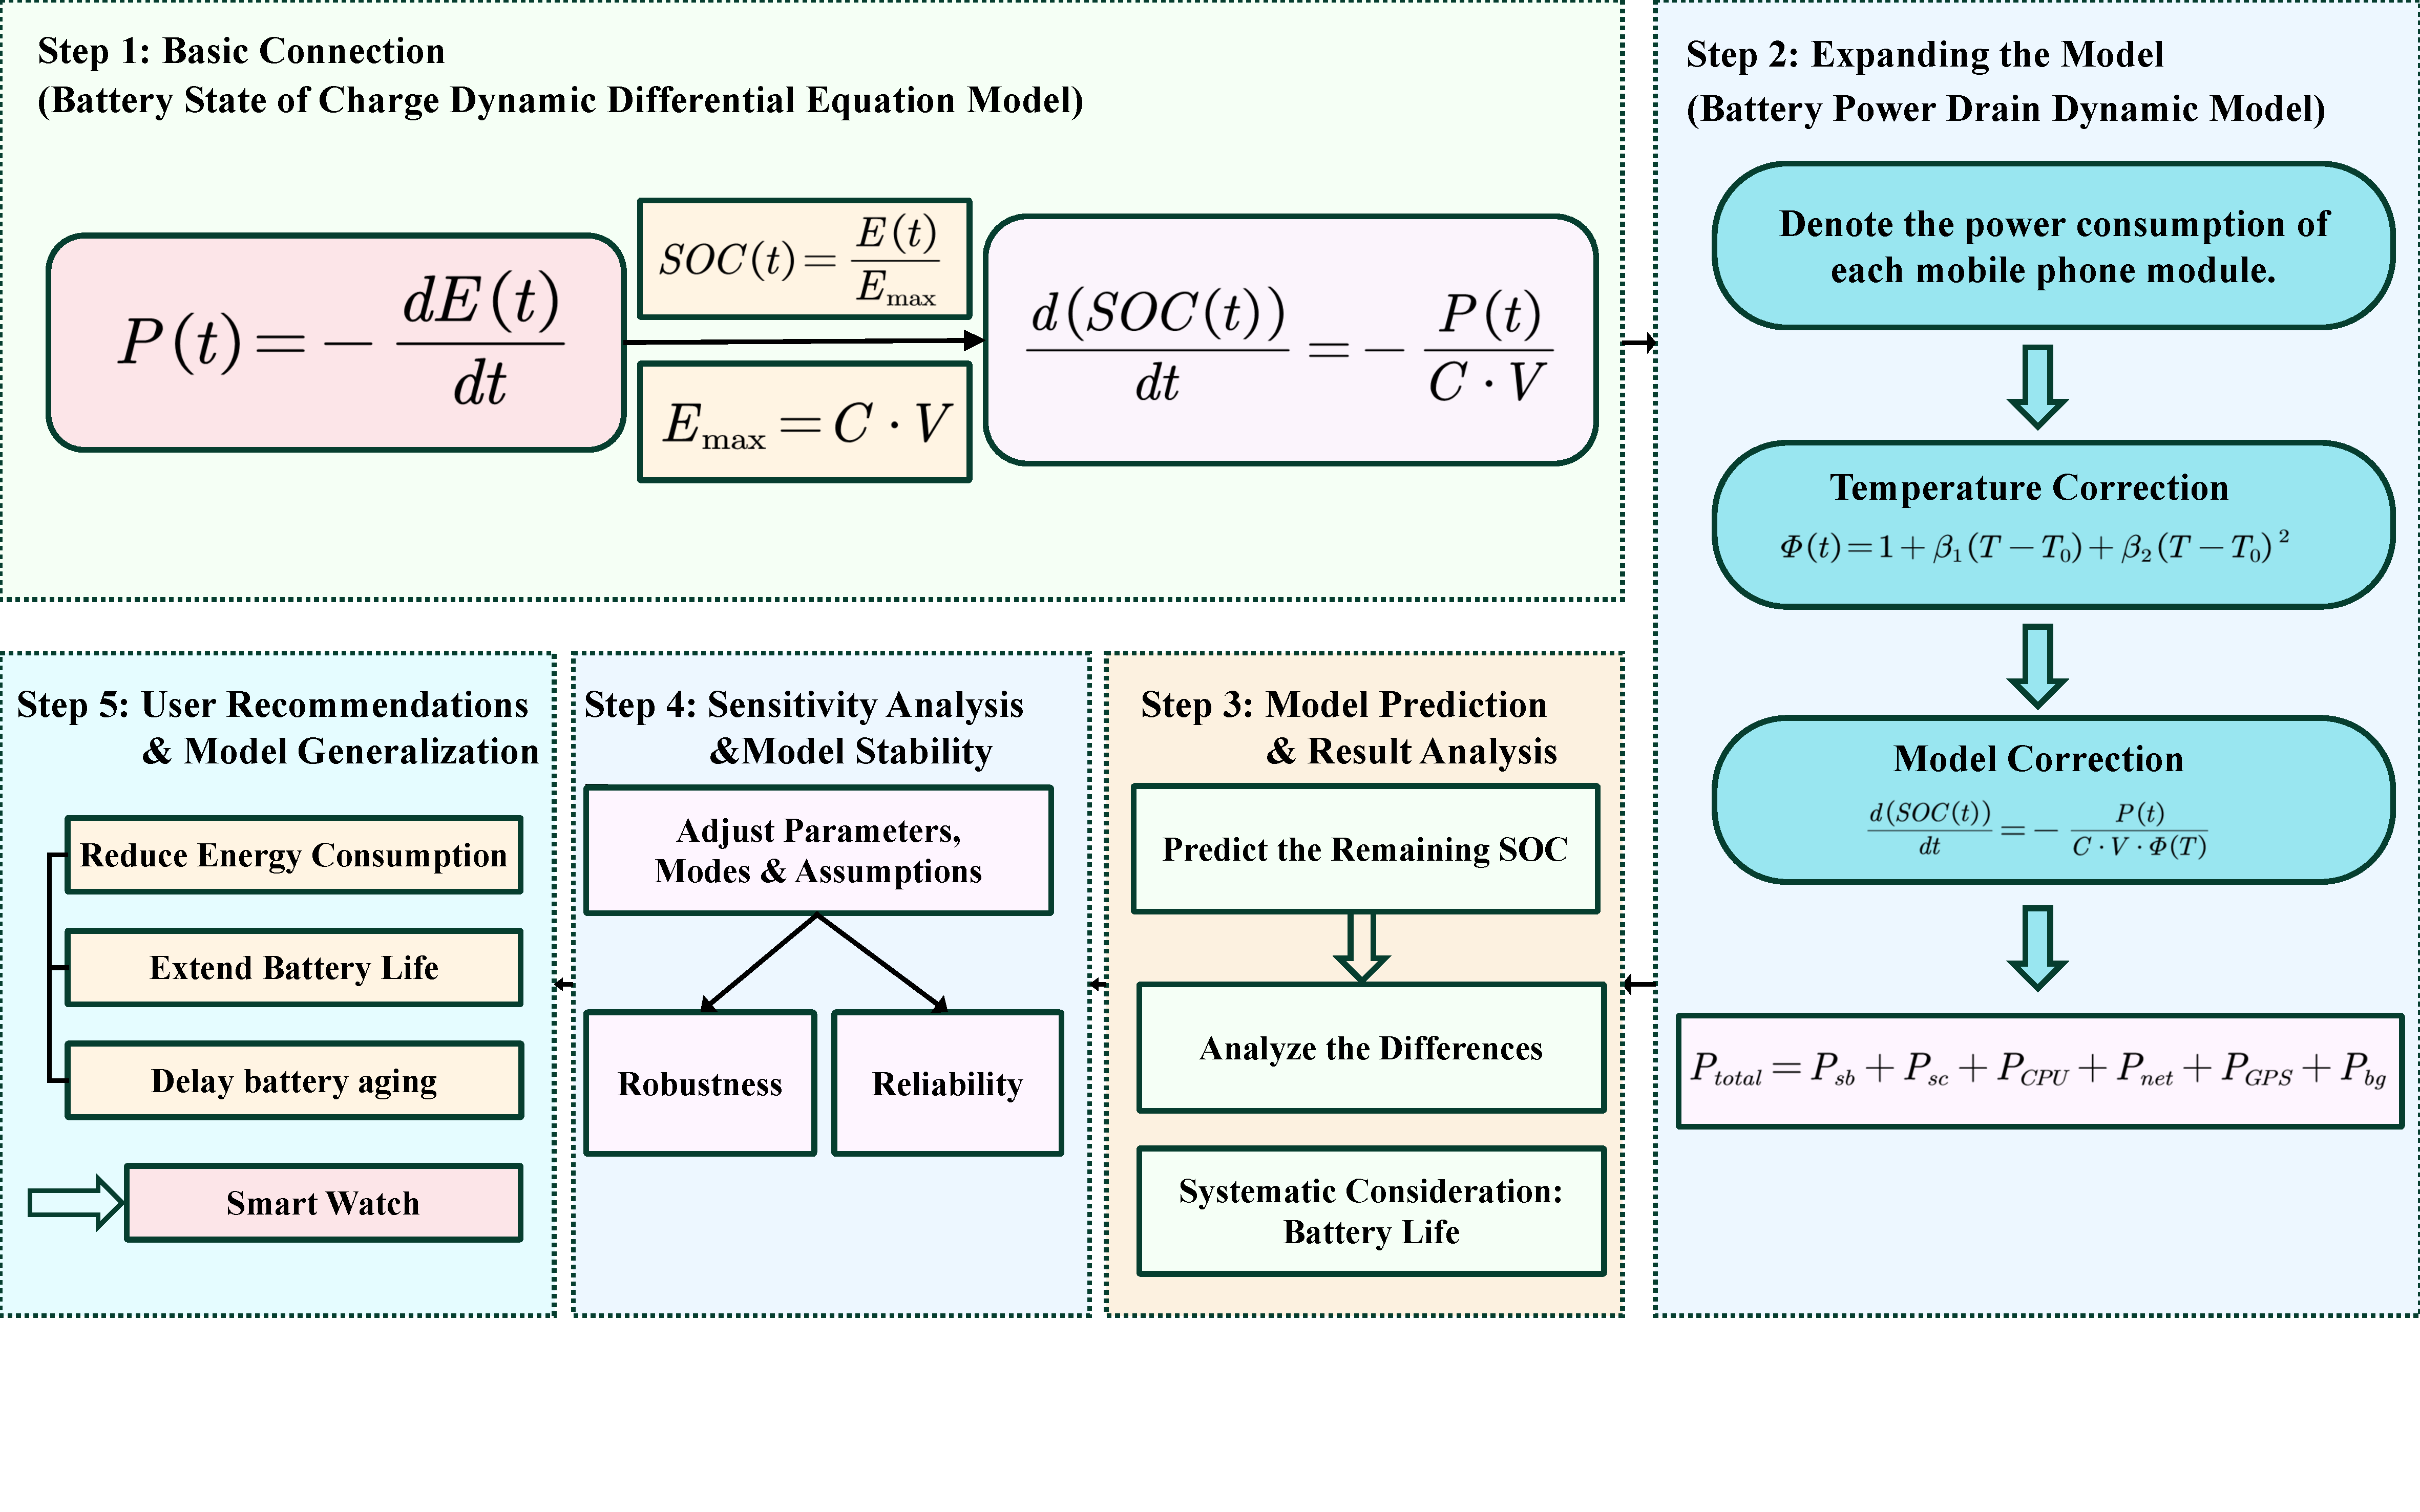
\includegraphics[
		width=1\textwidth,
		trim=0cm 5cm 0cm 0cm, 
		clip
		]{figures/2026美赛流程图.pdf}
		\caption{Flow Chart of Our Work}
		\label{fig:2026美赛流程图}
	\end{figure}
	
	
	\section{Assumptions and Justifications}  % 一级标题
	Considering that the problem may be very complex in the real situation, it’s necessary for us to make some reasonable assumptions first to simplify the problem. Each assumption is properly followed by the justification: 
	\begin{itemize}
		\item \textbf{Assumption:} 在建立模型时认为在相同使用场景时温度恒定 \\
		\textbf{Justification:} 在常规使用时间尺度内，智能终端具备有效散热能力，设备温度可视为在给定环境条件下近似恒定。
		
		\item \textbf{Assumption:} 使用OLED屏对剩余电量预测 \\
		\textbf{Justification:} 目前OLED屏较流行，预测结果贴合实际应用。
		
		\item \textbf{Assumption:} 固定网络环境分别估计剩余电量 \\
		\textbf{Justification:} 在实际应用中网络连接变换较少。
		
		\item \textbf{Assumption:} 不考虑模块间的耦合效应 \\
		\textbf{Justification:} 模块间的协同和抵消作用对功耗影响较小且会反应到各模块的功率消耗中。
		
		\item \textbf {假设：} 手机搭载锂离子电池。\\
		\textbf {依据：} 绝大多数现代智能手机均采用锂离子电池供电。
	\end{itemize}
	
	
	\section{Notations}  % 一级标题
	
	The key notations used in this paper are listed in Table 1.
	\begin{table}[h!]
		\centering
		\caption{本文使用的符号说明}
		\label{tab:notations}
		\renewcommand{\arraystretch}{1.5} 
		\begin{tabular}{lc}
			\toprule
			\textbf{符号} & \textbf{定义} \\
			\midrule
			\rowcolor{LightGreen}
			$SOC(t)$ & 时刻$t$时电池的荷电状态 \\
			$P(t)$ & 时刻$t$时的瞬时总功耗 \\
			\rowcolor{LightGreen}
			$C$ & 电池额定容量 \\
			$V$ & 电池标称电压 \\
			\rowcolor{LightGreen}
			$P_{module}$ & 手机各模块的功耗 \\
			$\alpha_{screen}$ & 屏幕功耗系数 \\
			\rowcolor{LightGreen}
			$B(t)$ & 归一化屏幕亮度 \\
			$\beta_{freq}$ & 与CPU利用率相关的动态功耗系数 \\
			\rowcolor{LightGreen}
			$\beta_{idle}$ & CPU空闲功耗 \\
			$u(t)$ & CPU利用率 \\
			\rowcolor{LightGreen}
			$r(t)$ & 时刻$t$时的网络数据传输速率 \\
			$\alpha_{net}$ & 动态功耗系数 \\
			\rowcolor{LightGreen}
			$\beta_{net}$ & 维持网络连接的基础功耗（无数据传输） \\
			$\delta_{\text{bg},0}$ & 后台基础功耗 \\
			\rowcolor{LightGreen}
			$\delta_{\text{bg},1}$ & 后台应用活动的动态功耗系数 \\
			$b(t)$ & 后台活动强度的无量纲描述符 \\
			\rowcolor{LightGreen}
			$\Phi(t)$ & 无量纲温度修正系数（系统在温度$T$与参考温度$T_0$下的性能比） \\
			$\beta$ & 温度系数 \\
			\rowcolor{LightGreen}
			$T$ & 电池当前工作温度 \\
			$T_0$ & 参考温度 \\
			\bottomrule
		\end{tabular}
	\end{table}
	
	\newpage
	
	\section{电池功率消耗动态微分方程模型} 
	
	为了使得模型更加符合实际情况，我们上网查阅了数据，修正模型系数，数据来源见表\ref{数据来源}。
	
	\begin{table}[htbp]
		\centering
		\caption{数据来源} % 明确标题
		\label{数据来源} % 规范标签
		\renewcommand{\arraystretch}{1.5}
		\renewcommand{\heavyrulewidth}{1.2pt}
		% 优化列宽，避免URL换行混乱
		\begin{tabular}{p{5cm}p{8cm}}
			\toprule
			数据类型 & 网址链接 \\
			\midrule
			屏幕发光特性数据 & \url{https://displaymate.com/Smartphone_ShootOut_1.htm?utm_source#Highlights} \\
			\midrule
			不同应用类别的后台功耗差异系数 & \url{https://www.phonearena.com/news/these-apps-silently-drain-your-smartphone-battery_id177012}
			\\
			\bottomrule
		\end{tabular}
		\renewcommand{\heavyrulewidth}{0.8pt}
	\end{table}
	
	\subsection{模型选择}
	\textbf{不选择电化学模型：}
	
	在电池建模领域，等效电路模型和电化学模型常用于描述端电压动态、极化效应和电池老化过程。然而，本题的建模目标并非对电池内部物理过程进行精确刻画，而是从用户使用行为出发，分析不同功能模块对电量消耗的影响及其对SOC 演化的作用。
	
	在实际使用场景中，用户侧可获得的信息主要是功能使用状态与功率消耗，而非电池端电压、电流或内部温度等状态量。因此，引入依赖于电流、电压的电池机理模型不仅难以参数标定，也会显著增加模型复杂度，降低模型的可解释性。
	
	\textbf{选择电池功率消耗动态微分方程模型：}
	
	为结合实际生活，数据能在实际应用中方便标定，本文采用基于能量守恒的一阶SOC演化模型，将重点放在功率项的结构化建模上，通过刻画屏幕、CPU、网络等模块的行为驱动功耗特性，实现对用户行为与电量消耗关系的有效描述。
	

	\subsection{综合考虑多因素的功耗函数}
	首先，由基本关系$SOC(t) = \frac{E(t)}{E_{\max}}$、$E_{\max} = C \cdot V$我们建立了初步的电池功率消耗的微分方程：
	\begin{equation}
		\frac{d(SOC(t))}{dt} = -\frac{P(t)}{C \cdot V}
	\end{equation}
	
	我们把总功率拆解为待机功率、屏幕使用功率、CPU 工作功率、网络工作功耗、GPS功耗及后台应用功耗：
	\begin{equation}
		P_{total}=P_{standby}+P_{screen}+P_{CPU}+P_{network}+P_{GPS}+P_{background}
	\end{equation}
	
	接下来，我们逐一明确各功率的组成：
	\begin{enumerate}[label=\arabic*.]
		\item \textbf{待机功率$P_{standby}$}
		
		待机功率是指手机在屏幕关闭、无主动用户操作条件下维持系统运行的基础功耗，与后台应用是否存在无关。有文献表明，手机闲置时的基础功率大约在268mW，可取0.27W作为接下来的进一步分析\upcite{1}，即：
		\begin{equation}
			P_{standby}=0.27W
		\end{equation}
		
		
		\item \textbf{屏幕使用功率 $P_{\text{screen}}$}
		屏幕功耗与亮度、亮屏时长显著正相关，针对主流的OLED、LCD屏分别构建功耗计算模型：
		\begin{enumerate}[label=(\arabic*)]
			\item \textbf{OLED}
			OLED为自发光器件，黑态显示像素关闭、功耗近0，高亮度高饱和度显示时像素全功率发光，功耗随显示内容的亮度、色彩占比大幅波动且与亮度正相关\upcite{2}；其像素发光功率与亮度呈非线性关系\upcite{3}，引入二次项$B(t)^2$拟合，同时考虑深色内容的节能效应，建立功耗模型如下：
			\begin{equation}
				P_{\text{screen,OLED}}(t) = \left( \alpha_{\text{OLED}} B(t) + \gamma_{\text{OLED}} B(t)^2 \right) \left( 1 - \eta k(t) \right)
			\end{equation}
			其中，$P_{\text{screen,OLED}}(t)$为时刻$t$OLED屏瞬时工作功率；$\alpha_{\text{OLED}}=0.7\mathrm{W}$、$\gamma_{\text{OLED}}=0.3\mathrm{W}$分别为亮度线性、非线性功耗系数；$\eta=0.8$为深色内容功耗衰减系数；$k(t)$为时刻$t$黑色像素占比，取值$[0,1]$；$B(t)$为时刻$t$归一化亮度值。模型简化为：
			\begin{equation}
				P_{\text{screen,OLED}}(t) =\left( 0.7B(t) + 0.3B(t)^2 \right) \left( 1 - 0.8k(t) \right)
			\end{equation}
			
			\item \textbf{LCD}
			LCD依赖LED背光层供光，像素仅调节透光率、背光层持续开启，功耗由背光亮度主导，全黑显示仍有基础背光功耗，屏幕功耗与亮度呈显著线性关系\upcite{4}，与屏幕面积相关性较弱，建立功耗模型如下：
			\begin{equation}
				P_{\text{screen,LCD}}(t) = \alpha_{\text{LCD}} B(t)
			\end{equation}
			其中，$P_{\text{screen,LCD}}(t)$为时刻$t$LCD屏瞬时工作功率；$\alpha_{\text{LCD}}=0.9\mathrm{W}$为亮度功耗系数；$B(t)$为时刻$t$归一化亮度值。模型简化为：
			\begin{equation}
				P_{\text{screen,LCD}}(t) = 0.9 B(t)
			\end{equation}
			
			\begin{figure}[h!]
				\centering
				\renewcommand{\arraystretch}{1}
				\subcaptionbox{Screen Power Consumption\label{fig:Screen Power Consumption}}%
				{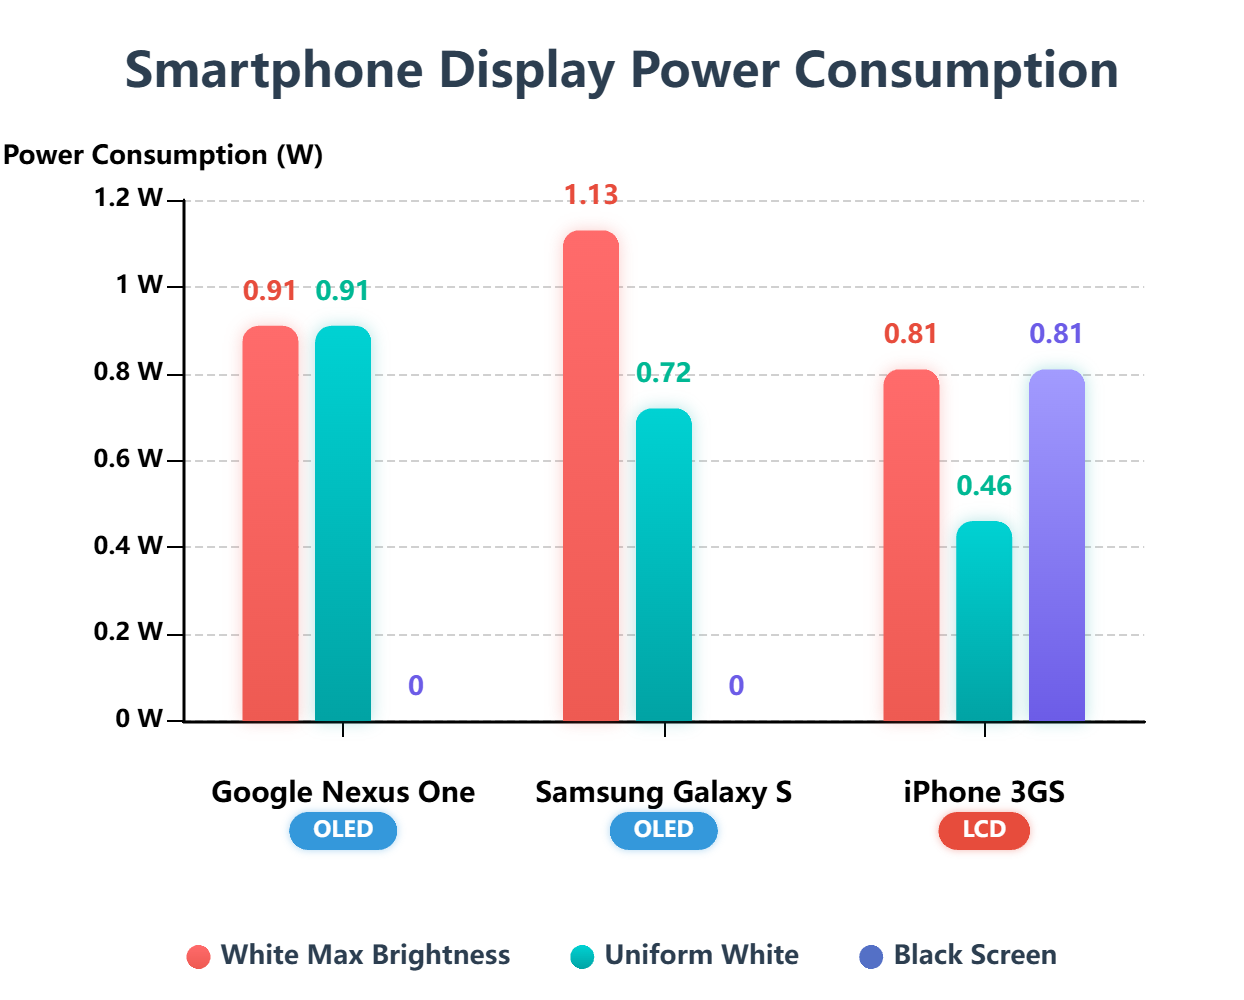
\includegraphics[width=.4\textwidth]{figures/OLED.png}}%
				\hspace{60pt} % 自定义间距，10pt约3.5mm
				\subcaptionbox{The common value of $B(t)$\label{fig:The common value of $B(t)$}}%
				{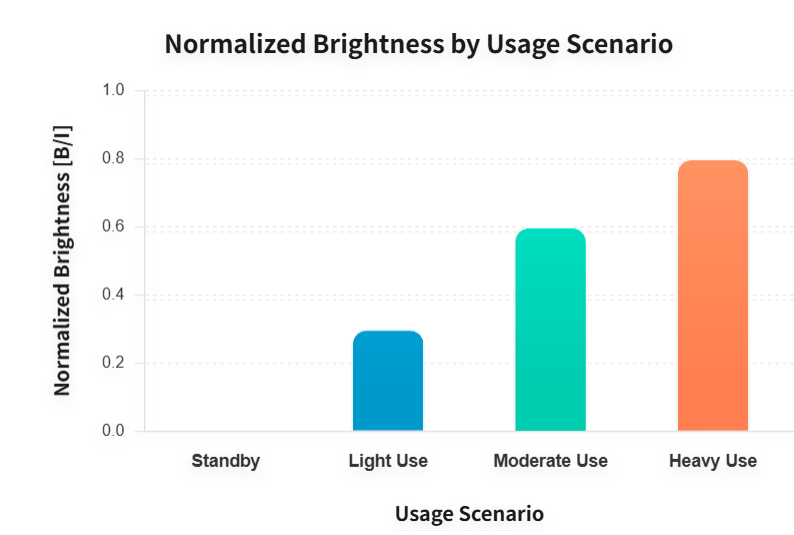
\includegraphics[width=.4\textwidth]{figures/B.png}}
				\renewcommand{\arraystretch}{1.5}
			\end{figure}
			
		\end{enumerate}
		
		\newpage
		
		\item \textbf{CPU工作功率$P_{CPU}$}
		
		CPU工作功率为处理器执行任务与运算时的功耗，其与CPU占用率（非空闲进程执行时长与总运行时长的比值）存在强关联，通过调控CPU占用率可建立其与功耗的量化关系，具体调控流程如图 \ref{fig:CPU}。
		\begin{figure}[h!]
			\centering
			% trim = 左边裁剪 下边裁剪 右边裁剪 上边裁剪（单位：cm）
			% clip 表示启用裁剪功能
			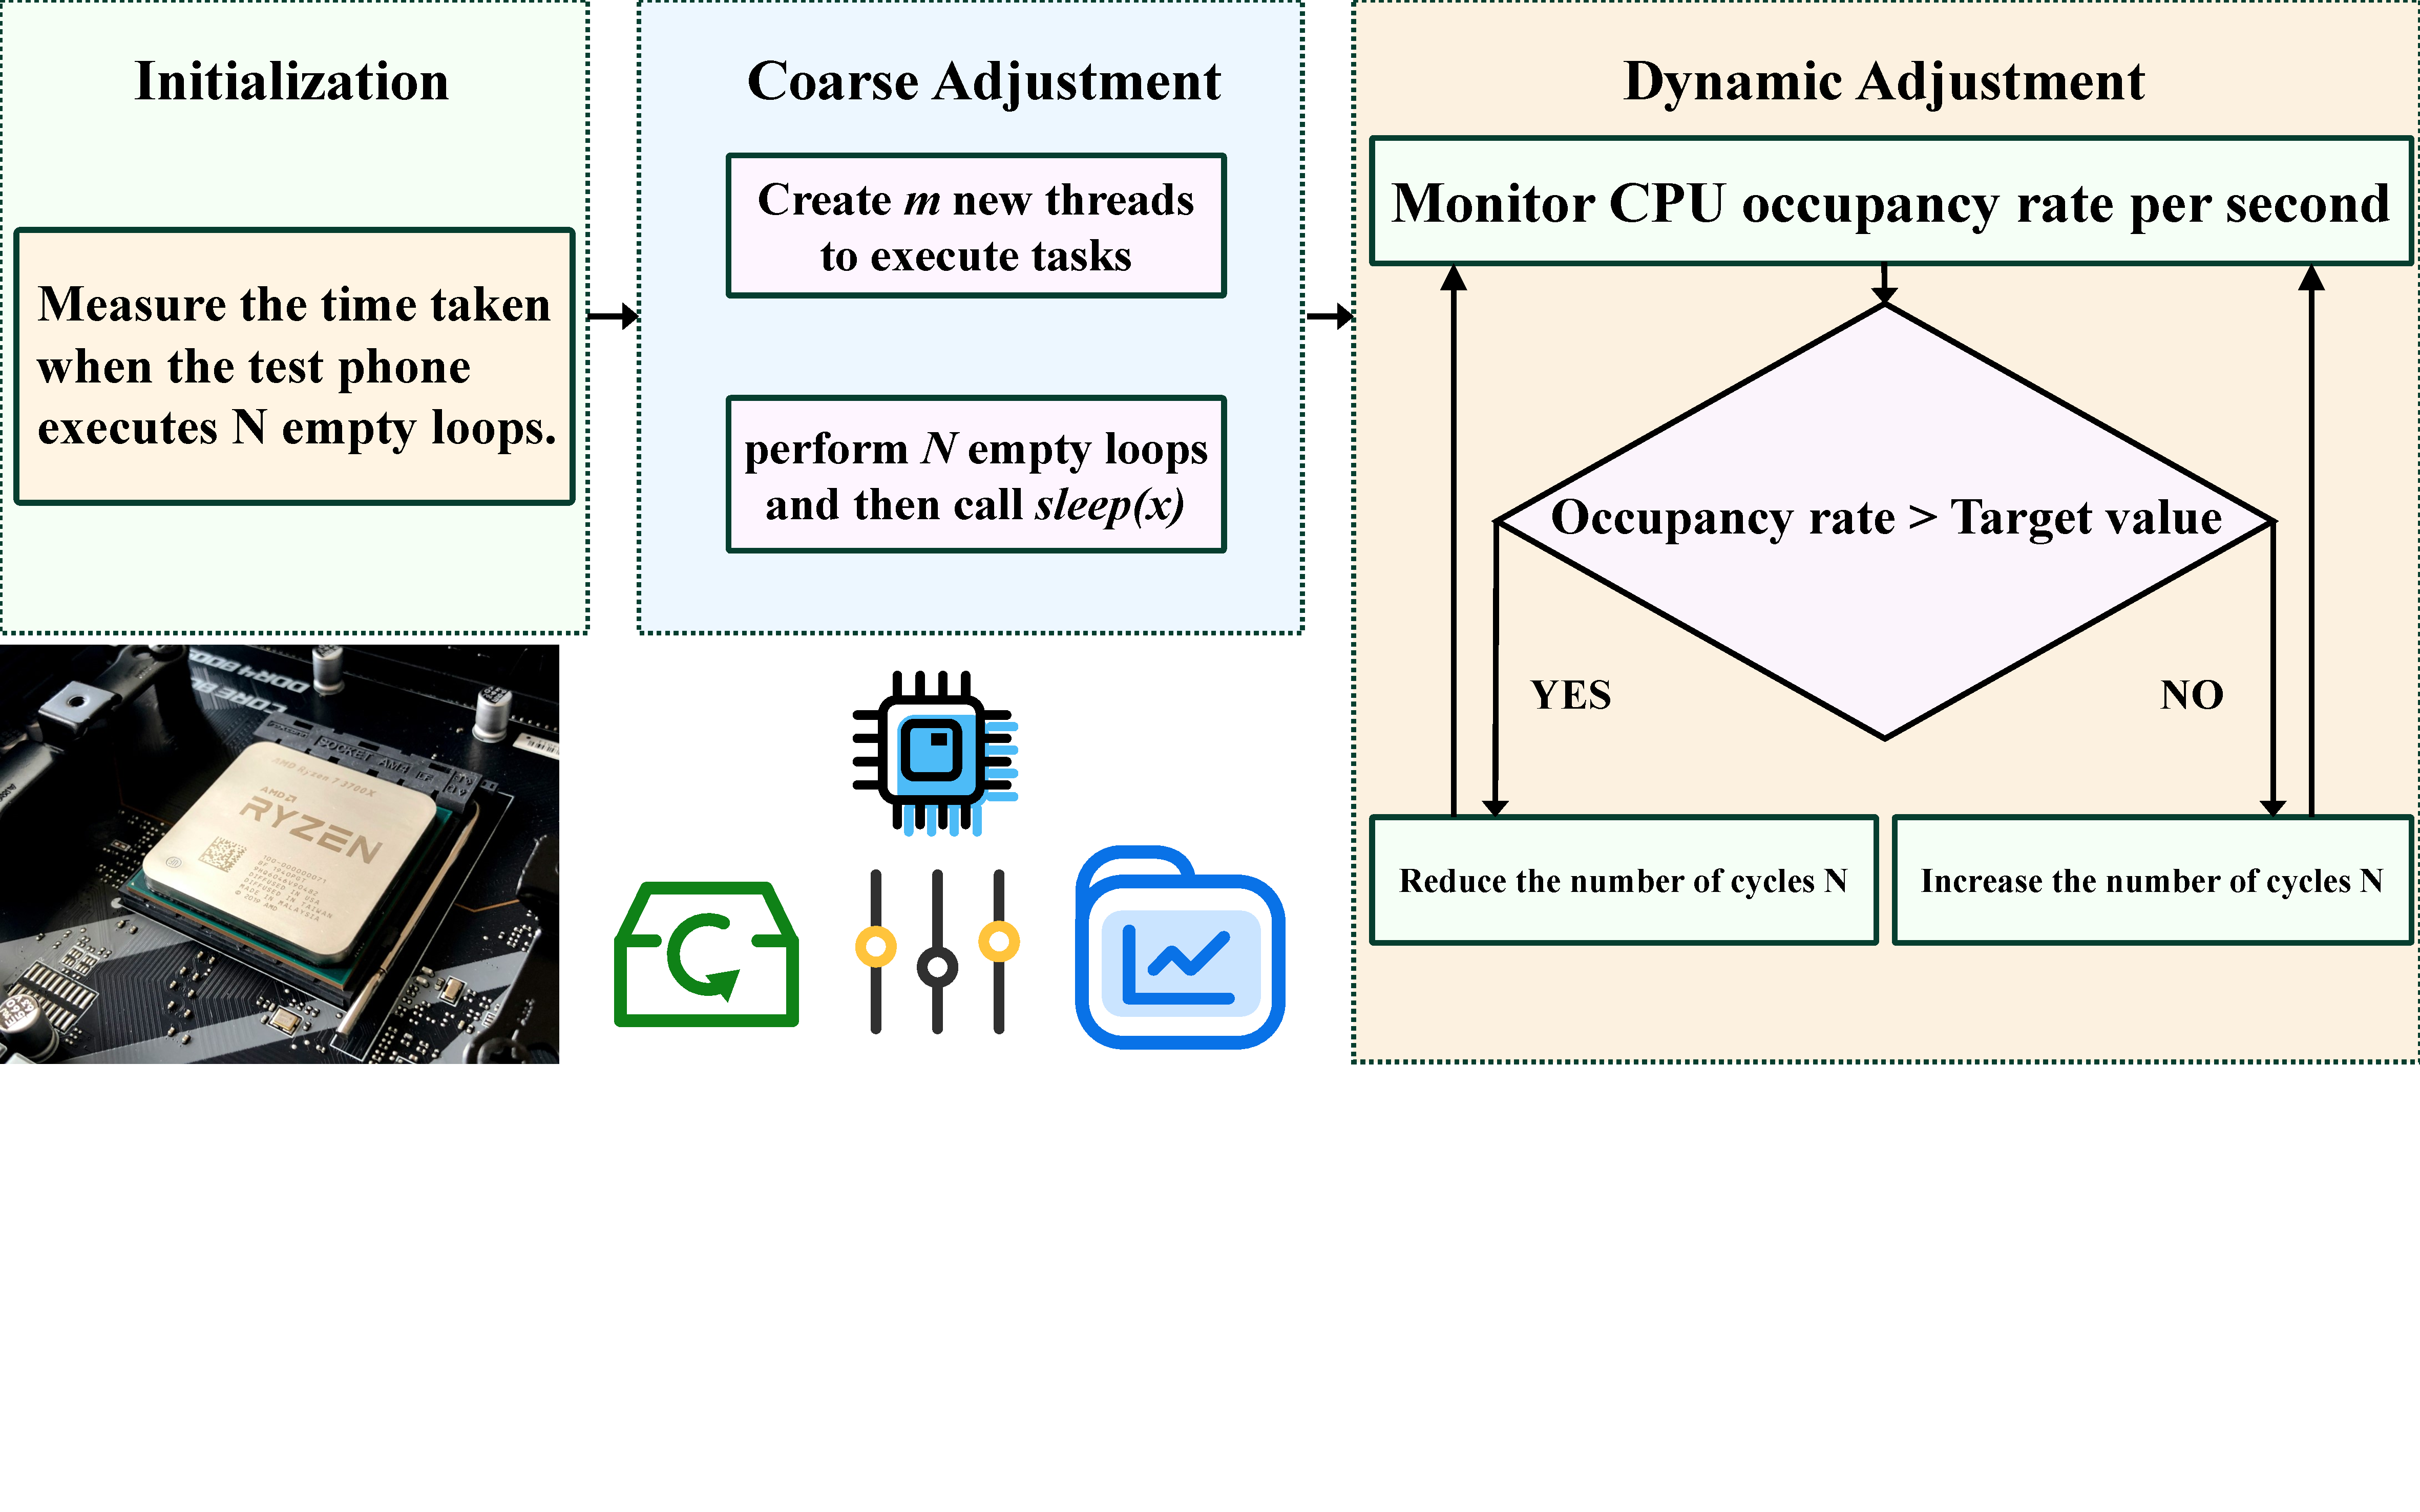
\includegraphics[
			width=1\textwidth,
			trim=0cm 14cm 0cm 0cm, 
			clip
			]{figures/CPU.pdf}
			\caption{CPU占用率控制流程}
			\label{fig:CPU}
		\end{figure}
		
		综上，构建CPU功耗模型如下：
		\begin{equation}
			P_{CPU}(t)=\beta_{freq}u(t)+\beta_{idle}
		\end{equation}
		其中，$P_{CPU}(t)$为CPU的即时功耗，$u(t)$是CPU的利用率，$u(t)\in[0,1]$，$\beta_{freq}$是与CPU利用率相关的动态功耗系数，$\beta_{idle}$是CPU空闲态功耗。根据现代手机功耗情况，取$\beta_{freq}=0.8W$,$\beta_{idle}=0.2W$\upcite{5}，则CPU功耗模型简化为：
		\begin{equation}
			P_{CPU}(t)=0.8u(t)+0.2
		\end{equation}
		
		\item \textbf{网络工作功率$P_{network}$}
		
		网络工作功率是手机通过移动网络、Wi-Fi 等进行数据传输、信号交互时产生的功率。经数据统计\upcite{6}，其功率模型采用线性拟合形式。我们考虑了不同类型网络连接（Wi-Fi、4G、5G）对应的不同功率特性，建立各网络类型的功率数学模型：
		
		\begin{equation}
			P_{\text{network}}(\tau(t)) = a_{network}\tau(t) + b_{network}
		\end{equation}
		
		其中，$P_{\text{network}}^{\text{network}}(\tau(t))$ 为网络的瞬时工作功率；$\tau(t)$ 网络负载强度（取值范围 $[0,1]$）；$a_{\text{network}}$ 为 Wi-Fi 网络负载功率系数，$b_{\text{network}}$ 为 Wi-Fi 网络基础工作功率，结合文献实测数据标定，取$a_{\text{Wi-Fi}}=0.18\mathrm{W}$，$b_{\text{Wi-Fi}}=0.08\mathrm{W}$，$a_{4\text{G}}=0.507\mathrm{W}$，$b_{4\text{G}}=0.15\mathrm{W}$，$a_{5\text{G}}=0.65\mathrm{W}$，$b_{5\text{G}}=0.15\mathrm{W}$。于是模型可简化为：
		
		\begin{equation}
			\begin{cases}
				P_{\text{network}}^{\text{Wi-Fi}}(\tau(t)) = 0.18\tau(t) + 0.08 \\
				P_{\text{network}}^{4\text{G}}(\tau(t)) = 0.507\tau(t) + 0.15 \\
				P_{\text{network}}^{5\text{G}}(\tau(t)) = 0.65\tau(t) + 0.15
			\end{cases}
		\end{equation}
		
		
		\item \textbf{GPS功耗 $P_{GPS}$}
		
		GPS 功耗是手机开启全球定位系统（GPS）模块进行定位、导航时产生的功耗，是手机位置服务场景下的核心功耗项之一。其功耗特性与定位模式直接相关：在高精度定位（如实时导航、轨迹记录）模式下，GPS 模块需持续接收卫星信号并进行解算，功耗维持在较高水平；在低功耗定位（如后台粗略定位、签到打卡）模式下，模块采用间歇性工作方式，功耗显著降低。我们考虑了GPS在不同工作状态下对功耗的影响，结合现代手机 GPS 模块的实际功率消耗特性，建立其数学模型如下\upcite{3}：
		\begin{equation}
			P_{\text{GPS}}(t) =
			\begin{cases}
				0, & \text{GPS off} \\
				0.0492, & \text{GPS on} \\
				0.4449, & \text{GPS fix}
			\end{cases}
		\end{equation}
		
		\item \textbf{后台应用功耗 $P_{\text{background}}$}
		
		后台应用功耗是智能手机后台驻留应用产生的隐性功耗，这类应用通过后台数据刷新、消息推送等操作产生持续耗电，其功耗与应用运行数量、类型显著相关，实时联网类应用后台功耗更高，也受应用唤醒频率、数据传输量直接影响。
		
		为贴合实际场景，本研究依据应用运行特征与后台功耗差异，将主流后台应用划分为游戏、社交、视频三大类，结合线性加权与归一化思想，构建普适性的后台应用功耗数学模型如下：
		\begin{equation}
			P_{\text{bg}}(t) = \delta_{bg,0} + \frac{\delta_{bg}}{N_{bg,\text{max}}} \left( \omega_g N_g(t) + \omega_s N_s(t) + \omega_v N_v(t) \right)
		\end{equation}
		
		其中，$\delta_{bg,0}$为基础后台功耗，表征系统后台机制的固定功耗项；$\frac{\delta_{bg}}{N_{bg,\text{max}}} \left( \omega_g N_g(t) + \omega_s N_s(t) + \omega_v N_v(t) \right)$ 为后台应用引入的功耗动态增量，反映由应用数量与类型带来的功耗变化；$N_g(t), N_s(t), N_v(t)$ 分别为时刻 $t$ 后台运行的游戏类、社交类、视频类应用数量，为模型核心输入变量；$\omega_g, \omega_s,\omega_v$分别为游戏类、社交类、视频类应用的功率权重系数，无量纲，用于量化不同应用类型对后台功耗的差异化影响。
		
		为提升模型的实际拟合度与可靠性，本研究基于表\ref{数据来源}中的公开实测数据，通过数据拟合与权重优化计算，确定三类应用的功率权重系数取值为：$(\omega_g, \omega_s, \omega_v) = (0.23, 0.32, 0.45)$。于是后台应用功耗最终模型：
		\begin{equation}
			P_{\text{bg}}(t) = \delta_{bg,0} + \frac{\delta_{bg}}{N_{bg,\text{max}}} \left( 0.23 N_g(t) + 0.32 N_s(t) + 0.45 N_v(t) \right)
		\end{equation}
		
		考虑到各模块的协同和抵消影响较小，且一定程度上体现在了各模块的变化，我们不研究模块之间的相互影响。
		
	\end{enumerate}
		
		\subsection{考虑温度影响的模型修正}
		
		考虑到温度对手机电池性能的影响是非线性的，特别是在高温和低温下性能衰减会加速，于是对模型引入温度修正项：
		\begin{equation}
			\frac{d\,\text{SOC}(t)}{dt} = -\frac{P_{\text{total}}(t)}{C \cdot V \cdot \Phi(T)}
		\end{equation}
		\begin{equation}
			\Phi(T) = 1 + \beta_1(T - T_0) + \beta_2(T - T_0)^2
		\end{equation}
		其中，$T$为电池当前工作温度，$T_0$为参考温度，取$25^\circ\text{C}$，$\Phi(T)$为温度修正系数，它是一个无量纲量，表示在当前温度$T$下，系统的实际性能相对于参考温度$T_0$下性能的变化比例。$\beta_1$和$\beta_2$分别为一次项和二次项温度系数，采用最小二乘法对实验数据进行二次多项式拟合。具体步骤为：
		
		\begin{enumerate}[label=\arabic*.]
			\item 将温度 $T$ 作为自变量，电池相对容量 $C(T)/C(T_0)$ 作为因变量
			\item 求解目标函数最小化：
			\[
			\min_{\beta_1,\beta_2} \sum_{i=1}^{n} \left[ \frac{C(T_i)}{C(T_0)} - \left(1 + \beta_1(T_i - T_0) + \beta_2(T_i - T_0)^2\right) \right]^2
			\]
			\item 通过对目标函数分别对$\beta_1$和$\beta_2$求偏导并令其为零，得到系数的正规方程组，进而求解最优估计值
		\end{enumerate}
		
		经数据拟合取$\beta_1=-0.004$，$\beta_2=-0.00006$，用于后续定量分析\upcite{7}。
	
	\subsection{利用Runge-Kutta法求解常微分方程数值解}
	
	综上，构建得到手机电池荷电状态变化的微分方程组如下：
	\begin{equation}
		\left\{
		\begin{aligned}
			&\frac{d\,\text{SOC}(t)}{dt} = -\frac{P_{\text{total}}(t)}{C \cdot V \cdot \Phi(T)}
			\\
			&P_{\text{total}}(t) = P_{\text{standby}} + P_{\text{screen}}(t) + P_{\text{CPU}}(t) + P_{\text{network}}(t) + P_{\text{GPS}}(t) + P_{\text{background}}(t) \\
			&P_{\text{standby}}=0.27W
			\\
			&P_{\text{screen,OLED}}(t) = \left( \alpha_{\text{OLED}} B(t) + \gamma_{\text{OLED}} B(t)^2 \right) \left( 1 - \eta k(t) \right)
			\\
			&P_{\text{screen,LCD}}(t) = \alpha_{\text{LCD}} B(t) 
			\\
			&P_{CPU}(t)=\beta_{freq}u(t)+\beta_{idle} 
			\\
			&P_{\text{network}}(\tau(t)) = a_{network}\tau(t) + b_{network}
			\\
			&P_{\text{GPS}}(t) =
			\begin{cases}
				0, & \text{GPS off} \\
				0.0492, & \text{GPS on} \\
				0.4449, & \text{GPS in navigation mode}
			\end{cases}
			\\
			&P_{\text{bg}}(t) = \delta_{bg,0} + \frac{\delta_{bg}}{N_{bg,\text{max}}} \left( \omega_g N_g(t) + \omega_s N_s(t) + \omega_v N_v(t) \right)
			\\
			&\Phi(T) = 1 + \beta_1(T - T_0) + \beta_2(T - T_0)^2
		\end{aligned}
		\right.
	\end{equation}
	
	将相关参数代入后，可得定参后的微分方程组：
	\begin{equation}
		\left\{
		\begin{aligned}
			&\frac{d\,\text{SOC}(t)}{dt} = -\frac{P_{\text{total}}(t)}{C \cdot V \cdot \Phi(T)} 
			\\
			&P_{\text{total}}(t) = P_{\text{standby}} + P_{\text{screen}}(t) + P_{\text{CPU}}(t) + P_{\text{network}}(t) + P_{\text{GPS}}(t) + P_{\text{background}}(t) 
			\\
			&P_{\text{standby}}= 0.27W\\
			&P_{\text{screen,OLED}}(t) =\left( 0.7B(t) + 0.3B(t)^2 \right) \left( 1 - 0.8k(t) \right) 
			\\
			&P_{\text{screen,LCD}}(t) = 0.9 B(t)
			\\
			&P_{CPU}(t)=0.8u(t)+0.2 
			\\
			&P_{\text{network}}^{\text{Wi-Fi}}(\tau(t)) = 0.18\tau(t) + 0.08
			\\
			&P_{\text{network}}^{4\text{G}}(\tau) = 0.507\tau(t) + 0.15  
			\\
			&P_{\text{network}}^{5\text{G}}(\tau(t)) = 0.65\tau(t) + 0.15
			\\
			&P_{\text{GPS}}(t) =
			\begin{cases}
				0, & \text{GPS off} \\
				0.0492, & \text{GPS on} \\
				0.4449, & \text{GPS in navigation mode}
			\end{cases}
			\\
			&P_{\text{bg}}(t) = \delta_{bg,0} + \frac{\delta_{bg}}{N_{bg,\text{max}}} \left( 0.23 N_g(t) + 0.32 N_s(t) + 0.45 N_v(t) \right)
			\\
			& \Phi(T) = 1 + 0.004(T - T_0) + 0.00006(T - T_0)^2,\quad \Phi(T) > 0
		\end{aligned}
		\right.
	\end{equation}
	
	\begin{equation}
		T_{\text{battery life}} = \int_{0}^{\text{SOC}_0} \frac{C \cdot V \cdot \phi(T)}{P_{\text{total}}(t)} \, d(\text{SOC})
	\end{equation}
	
	我们采用四阶龙格--库塔（RK）方法求解该微分方程。作为一种适用于无解析解方程的单步数值方法，它通过对离散点斜率的加权平均实现高精度逼近，无需计算高阶导数。仅通过多次计算方程右侧函数的值，即可获得离散节点处的数值解\upcite{8}。其\textbf{四阶精度}满足电池功耗建模的工程精度要求。RK方法仅需计算\( P(t) \)函数值即可求解由多个模块叠加的非线性函数（无需解析导数），具有\textbf{计算成本低}、单步求解\textbf{无需历史数据}以及\textbf{稳定性强}的特点，能有效避免显式欧拉法在长期积分和随机扰动下的数值不稳定性。
	

	\subsection{随机仿真}
	为贴合实际场景，本研究基于美国市场主流手机参数（电池容量4000 mAh、标称电压3.8 V），选取电池最佳工作温度，固定网络模式为WiFi、4G、5G，对所建模型开展随机仿真测试。首先将其余功耗影响因素设为每20分钟同步随机变化，仿真结果见图\ref{fig:同步变化的随机仿真}，相关性能指标如表\ref{tab:controlled_comparison}所示。
	
	\begin{table}[h!]
		\centering
		\caption{同步变化的随机仿真}
		\label{tab:controlled_comparison}
		\renewcommand{\arraystretch}{1.5} 
		\begin{tabular}{lccc}
			\toprule
			\textbf{指标} & \textbf{Wi-Fi} & \textbf{4G} & \textbf{5G} \\
			\midrule
			\rowcolor{LightGreen}
			总放电时间 (h) & 10.66 & 9.51 & 9.18 \\
			平均SOC衰减速率 (h$^{-1}$) & 0.0938 & 0.1051 & 0.1089 \\
			\rowcolor{LightGreen}
			50\% SOC放电时间 (h) & 5.66 & 5.15 & 5.02 \\
			\bottomrule
		\end{tabular}
	\end{table}
	
	\begin{figure}[h!]
		\centering
		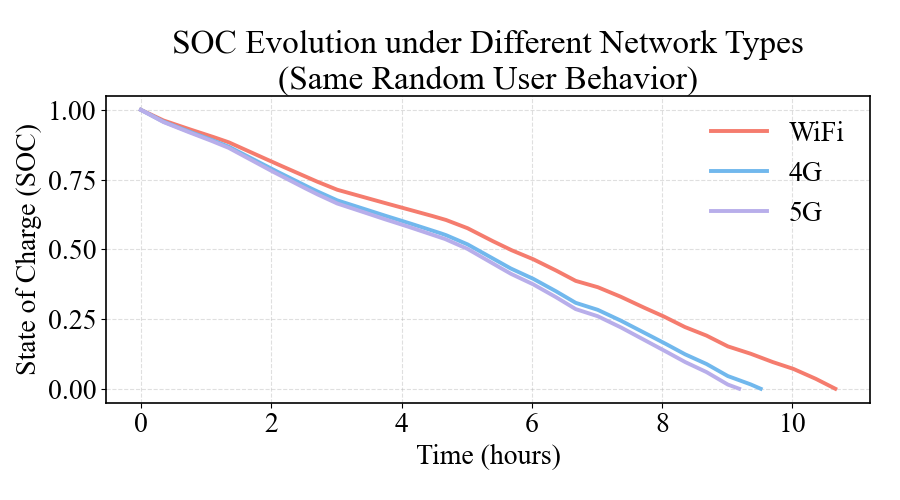
\includegraphics[width=0.8\textwidth,trim=0cm 0.4cm 0cm 0cm,clip]{figures/同步变化的随机仿真.png}
		\caption{同步变化随机仿真结果}
		\label{fig:同步变化的随机仿真}
	\end{figure}
	
	由图\ref{fig:同步变化的随机仿真}可知，各网络模式下电池SOC随时间持续下降，5G衰减最快、4G次之、WiFi最慢，该规律在放电全程稳定且无曲线交叉，与实际场景高度契合。其余能耗项一致，结果差异可明确归因于网络制式功耗不同：WiFi短距离、低发射功率实现低功耗，蜂窝网络需持续与基站信令交互，5G高吞吐特性进一步提升能耗。
	
	在此基础上开展二次仿真，保持温度与网络模式不变，将其余功耗影响因素设为每20分钟非同步独立随机变化，结果见图\ref{fig:独立变化的随机仿真}、表\ref{tab:realistic_comparison}。
	
	\begin{table}[h!]
		\centering
		\caption{独立变化的随机仿真}
		\label{tab:realistic_comparison}
		\renewcommand{\arraystretch}{1.5} 
		\begin{tabular}{lccc}
			\toprule
			\textbf{指标} & \textbf{Wi-Fi} & \textbf{4G} & \textbf{5G} \\
			\midrule
			\rowcolor{LightGreen}
			总放电时间 (h) & 10.92 & 9.72 & 9.23 \\
			平均SOC衰减速率 (h$^{-1}$) & 0.0915 & 0.1028 & 0.1083 \\
			\rowcolor{LightGreen}
			50\% SOC放电时间 (h) & 5.40 & 4.95 & 4.70 \\
			\bottomrule
		\end{tabular}
	\end{table}
	
	\begin{figure}[h!]
		\centering
		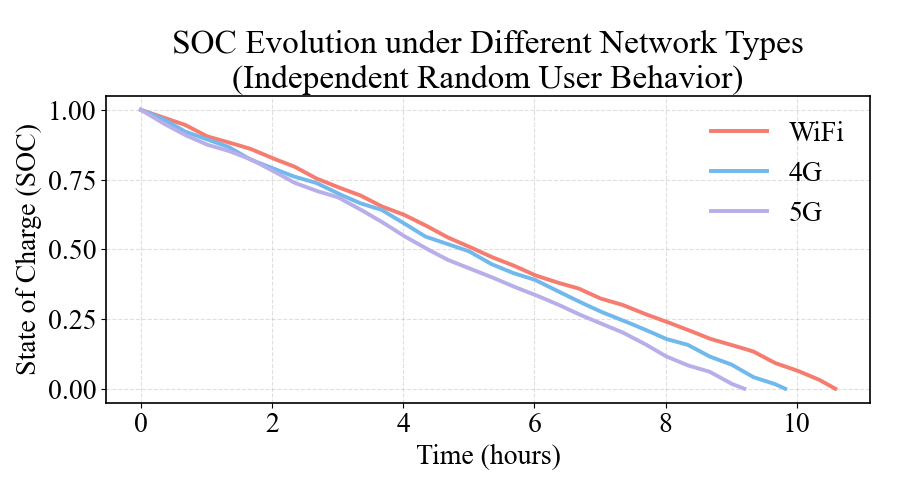
\includegraphics[width=0.8\textwidth,trim=0cm 0.4cm 0cm 0cm,clip]{figures/独立变化的随机仿真.png}
		\caption{独立变化随机仿真结果}
		\label{fig:独立变化的随机仿真}
	\end{figure}
	
	与同步仿真相比，SOC曲线随机波动更显著，4G衰减速率在部分时段短暂超过5G；但从整体来看，5G仍最先放电至0\%SOC，4G次之、WiFi最后，说明网络制式对能耗的影响在长时间统计下占主导。模型引入多源随机扰动后仍保持稳定能耗排序，体现出良好的鲁棒性。
	
	
	\subsection{参数估计方法与模型合理性说明}
	
	\begin{enumerate}[label=\arabic*.]
		\item \textbf{常用参数估计方法及其不适用性}
		
		系统建模与参数标定中，常用估计方法包括最大似然估计（MLE）、普通最小二乘法（OLS）、贝叶斯估计、梯度下降、遗传算法等优化方法。
		
		\textbf{未采用原因}：
		\begin{enumerate}[label=(\arabic*)]
			\item 数据稀缺与结构复杂：手机功耗为多因素耦合的复杂大系统，实际场景中难收集各模块同步功耗数据；模型为多变量非线性微分方程，传统拟合方法（如OLS）需大量时序数据，易受噪声干扰致结果不稳定；贝叶斯估计等需可靠数据支撑先验/后验分布，不适用。
			\item 模型物理意义优先于纯数据驱动：模型强调可解释性与物理一致性（如屏幕功耗-亮度非线性关系、CPU功耗-占用率线性关系均有硬件特性文献支撑）；机器学习方法为“黑箱”模型，无法解释参数物理意义，小样本易过拟合。
			\item 文献数据作为先验知识的主导作用：各模块功耗系数（如$\alpha_{\text{OLED}}=0.7\text{W}$、$\beta_{\text{freq}}=0.8\text{W}$）已有大量实验研究支撑，直接采用文献值可保证模型基本合理性，避免从零估计导致的大幅偏差。
		\end{enumerate}
		
		\item \textbf{基于归一化行为变量的参数标定方法}
		
		针对大规模实测数据缺失的情况，本研究采用基于归一化行为变量的参数标定方法。该方法首先将无法直接测量的行为变量（如屏幕亮度、CPU占用率、网络负载）归一化至$[0,1]$区间以消除量纲；随后，通过模块化方式构建各功耗模型，其系数来源于文献实测数据的均值或拟合结果，确保模型各部分具有明确的物理意义；最后，为避免机器学习方法对标注数据量大、泛化能力弱及参数缺乏物理解释等局限，本方法选择以机理驱动为基础，兼顾可解释性与工程适用性。
		
		\item \textbf{实测数据修正与参数确定规范}
		
		模型中的关键数据来源明确，遵循以下规范：
		\begin{enumerate}[label=(\arabic*)]
			\item 数据筛选与验证：优先选取近年发表、实验条件明确、样本量充足的文献数据；对不同来源数据进行交叉验证，剔除明显异常值。
			\item 参数拟合与确定：线性关系显著的模块（如LCD屏、CPU空闲功耗）直接采用文献报道典型值；非线性部分（如OLED屏亮度-功耗关系）采用二次项拟合，系数$\alpha_{\text{OLED}}=0.7$、$\gamma_{\text{OLED}}=0.3$通过OLS拟合文献数据获得；温度修正系数$\beta=-0.004$取自锂电池温度效应实验统计结果。
			\item 模型修正与验证：通过随机仿真验证模型输出与实际经验是否一致（如5G功耗$>$4G$>$Wi-Fi）；通过控制变量仿真验证各模块功耗贡献排序是否符合常识。
		\end{enumerate}
	\end{enumerate}
	
	
	
	\section{剩余电量预测与不确定性量化}  % 一级标题
	
	\subsection{剩余电量预测}
	
	我们考虑了生活中的大部分情况，在接下来的分析中固定网络连接为WiFi，模拟5种使用手机的场景，在不同场景下的指标如表\ref{tab:指标}所示：
	
	\newpage
	
	\begin{table}[h!]
		\centering
		\renewcommand{\arraystretch}{1.5}
		\caption{设备使用模式与参数对应表}
		\label{tab:指标}
		\begin{tabular}{lccccc}  % 改为5列
			\toprule
			使用模式 & $B(t)$ & $u(t)$ & $\tau$ & $P_{GPS}$ & $P_{background}$ \\
			\midrule
			\rowcolor{pink}
			待机     & 0   & 0    & 0 & 0.049 & 0.08 \\
			轻度使用 & 0.3 & 0.25 & 0.2 & 0.049 & 0.09 \\
			\rowcolor{pink}
			中度使用 & 0.6 & 0.55 & 0.6 & 0.049 & 0.09 \\
			重度使用 & 0.8 & 0.9  & 1 & 0.049 & 0.11 \\
			\rowcolor{pink}
			导航模式 & 0.6 & 0.55 & 0.6 & 0.45  & 0.09 \\  
			\bottomrule
		\end{tabular}
	\end{table}
	
	首先我们定初始电量为100\%，模拟各个场景的SOC变化，如图\ref{fig:100}所示，随后挑选了中度使用的场景模拟了在不同初始电量情况下的放电过程，如图\ref{fig:situation}所示：
	\begin{figure}[h!]
		\centering
		\renewcommand{\arraystretch}{1}
		\subcaptionbox{Screen Power Consumption\label{fig:100}}%
		{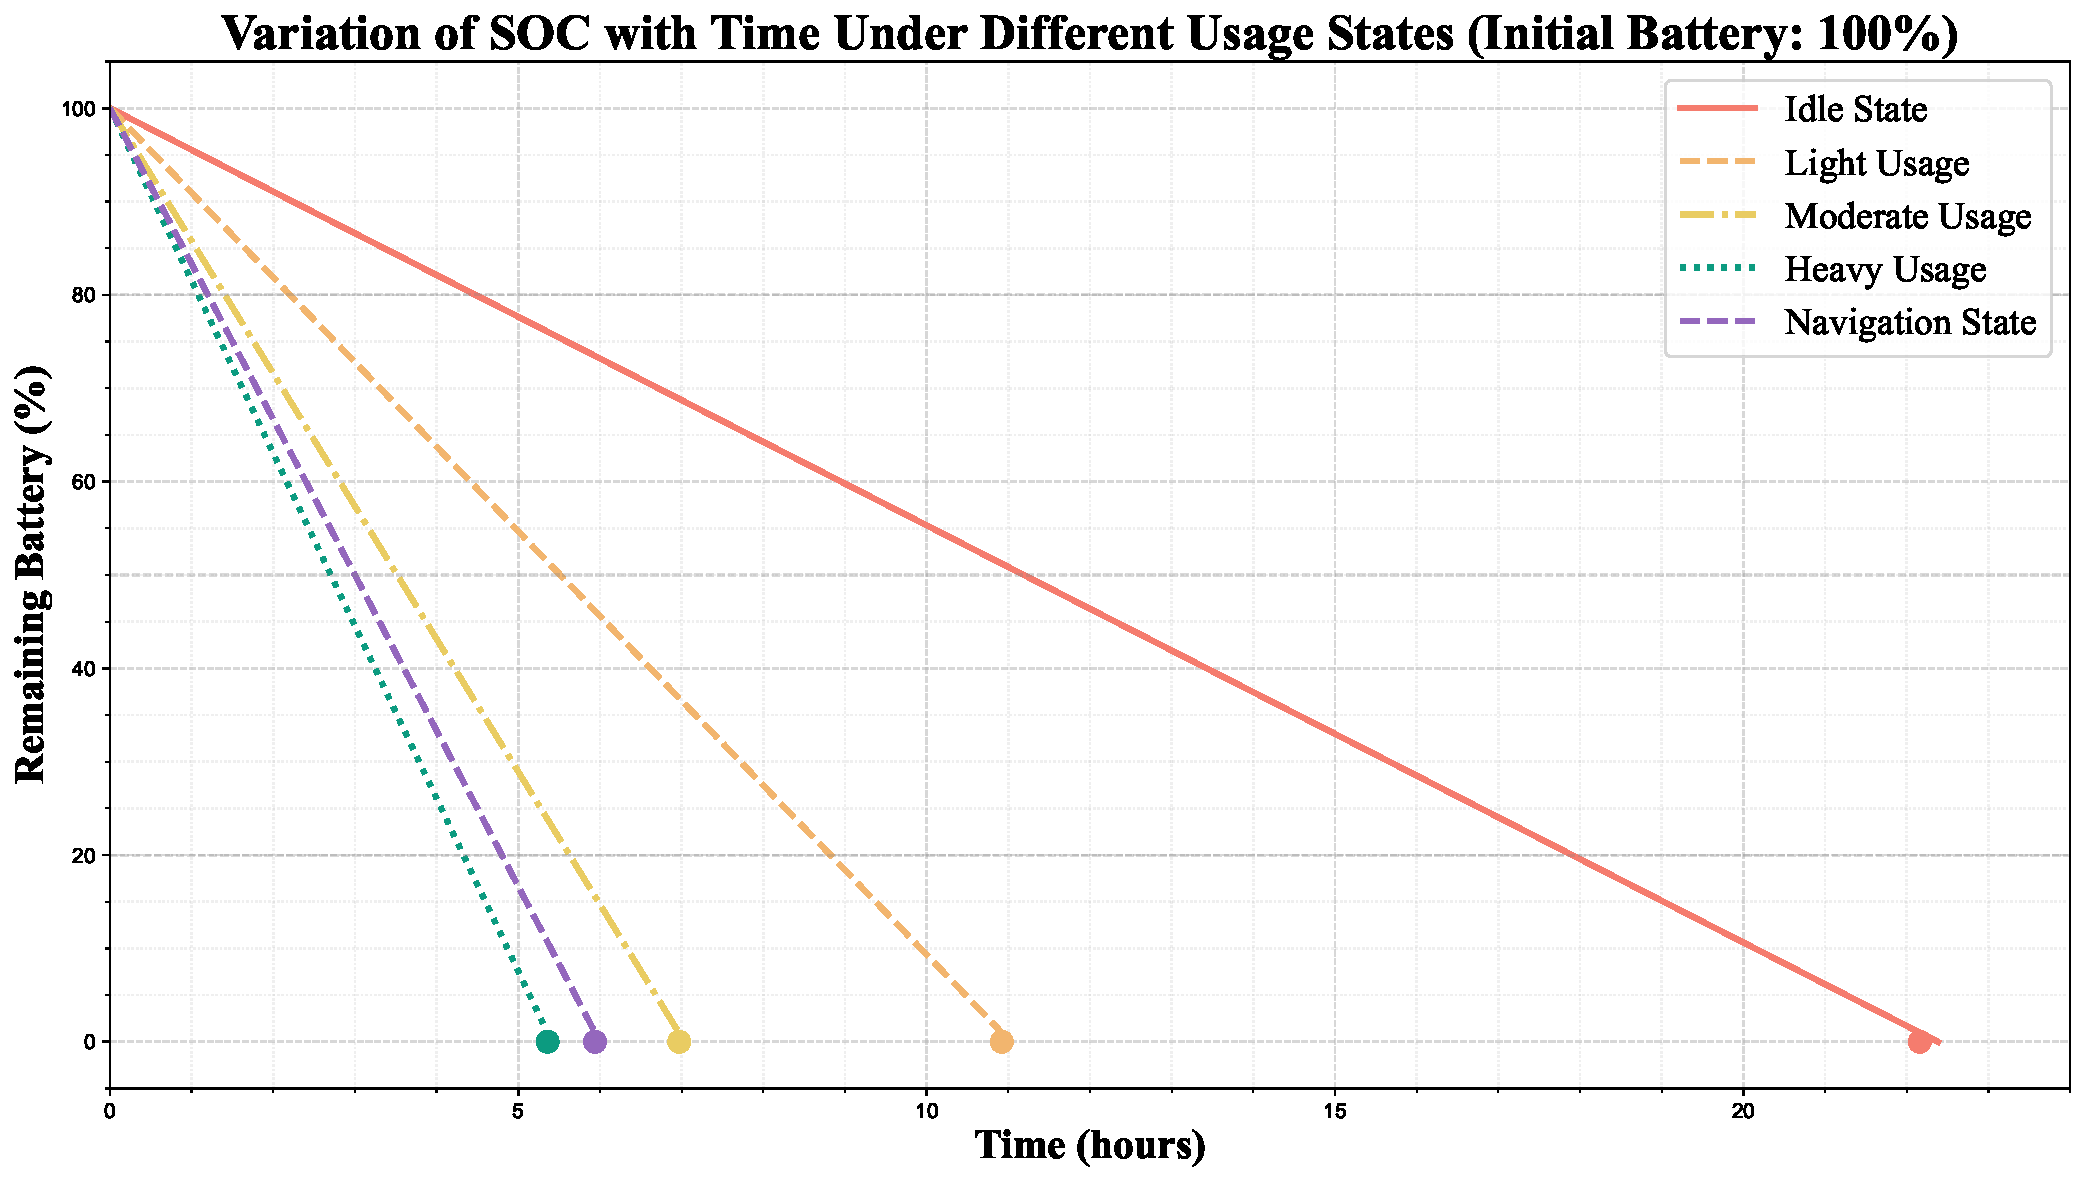
\includegraphics[width=.35\textwidth]{figures/100.pdf}}%
		\hspace{60pt} % 自定义间距，10pt约3.5mm
		\subcaptionbox{The common value of $B(t)$\label{fig:situation}}%
		{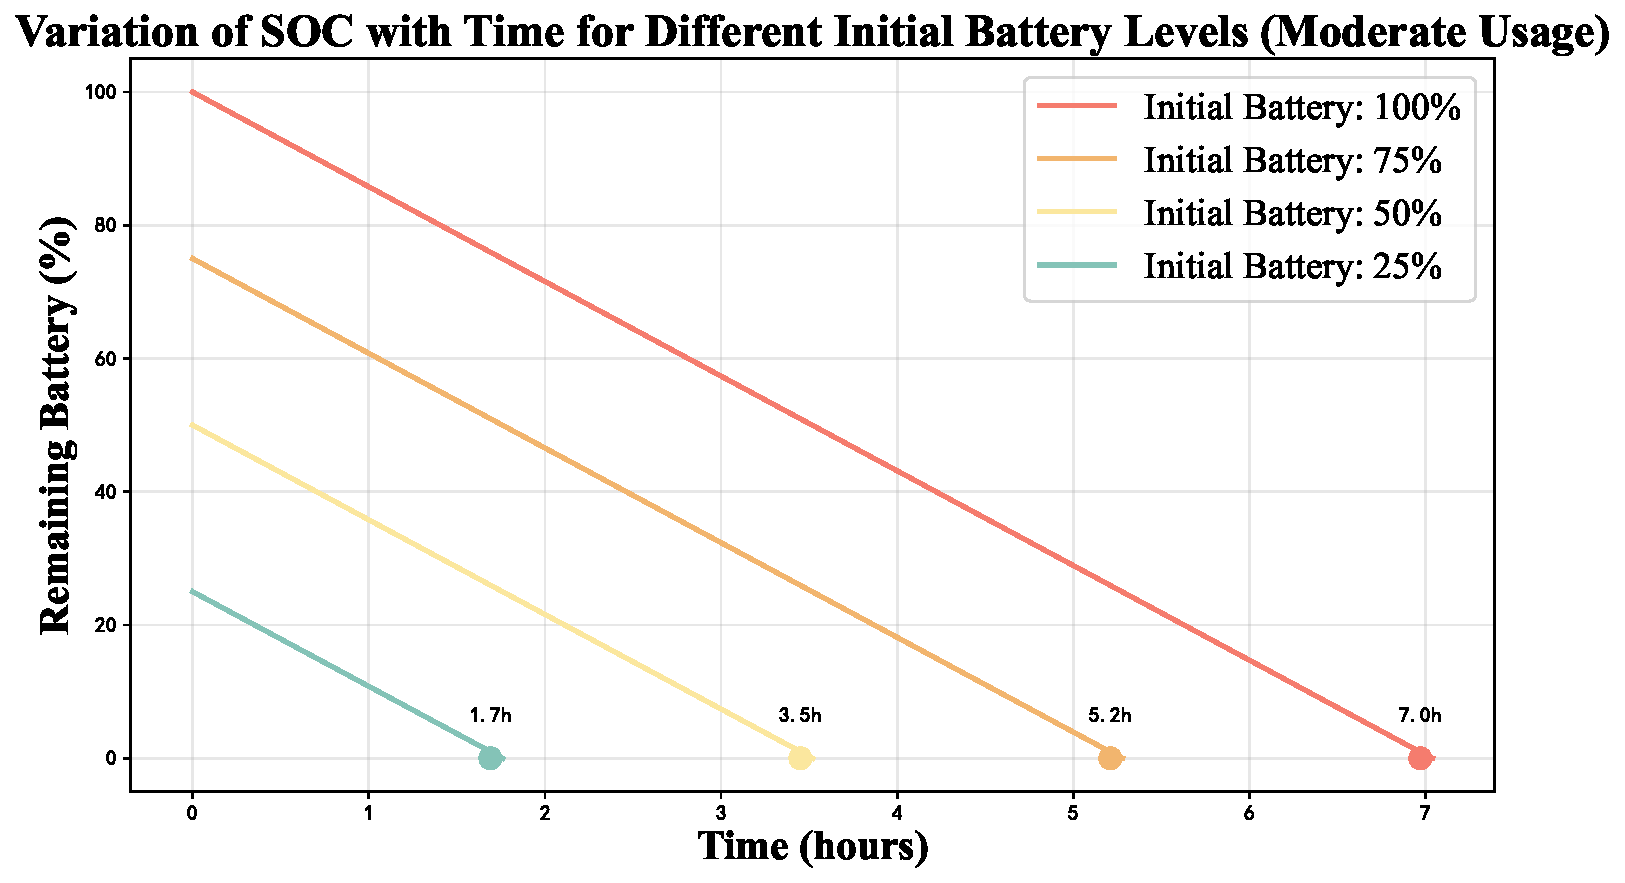
\includegraphics[width=.35\textwidth]{figures/situation.pdf}}
		\caption{}
		\renewcommand{\arraystretch}{1.5}
	\end{figure}
	
	\begin{table}[h!]
		\centering
		\renewcommand{\arraystretch}{1.5}
		\caption{不同使用状态下电池放电时长(小时)}
		\label{tab:all}
		\begin{tabular}{lcccc}
			\toprule
			State & 25\% & 50\% & 75\% & 100\% \\
			\midrule
			\rowcolor{pink}
			Idle State & 5.38 & 10.97 & 16.57 & 22.16 \\
			Light Usage & 2.65 & 5.41 & 8.17 & 10.92 \\
			\rowcolor{pink}
			Moderate Usage & 1.69 & 3.45 & 5.21 & 6.97 \\
			Heavy Usage & 1.30 & 2.66 & 4.01 & 5.36 \\
			\rowcolor{pink}
			Navigation State & 1.44 & 2.94 & 4.44 & 5.94 \\
			\bottomrule
		\end{tabular}
	\end{table}
		5种场景中，电池从100\%放电至0\%的时间如表\ref{tab:all}所示。5种场景的手机中各个模块消耗的功率如图\ref{fig:功率}所示，在中度使用的场景下，手机的各个模块功率关于总功率的占比见图\ref{fig:饼状图}：
		
		\newpage
		
	\begin{figure}[h!]
		\centering
		\renewcommand{\arraystretch}{1}
		\subcaptionbox{Screen Power Consumption\label{fig:功率}}%
		{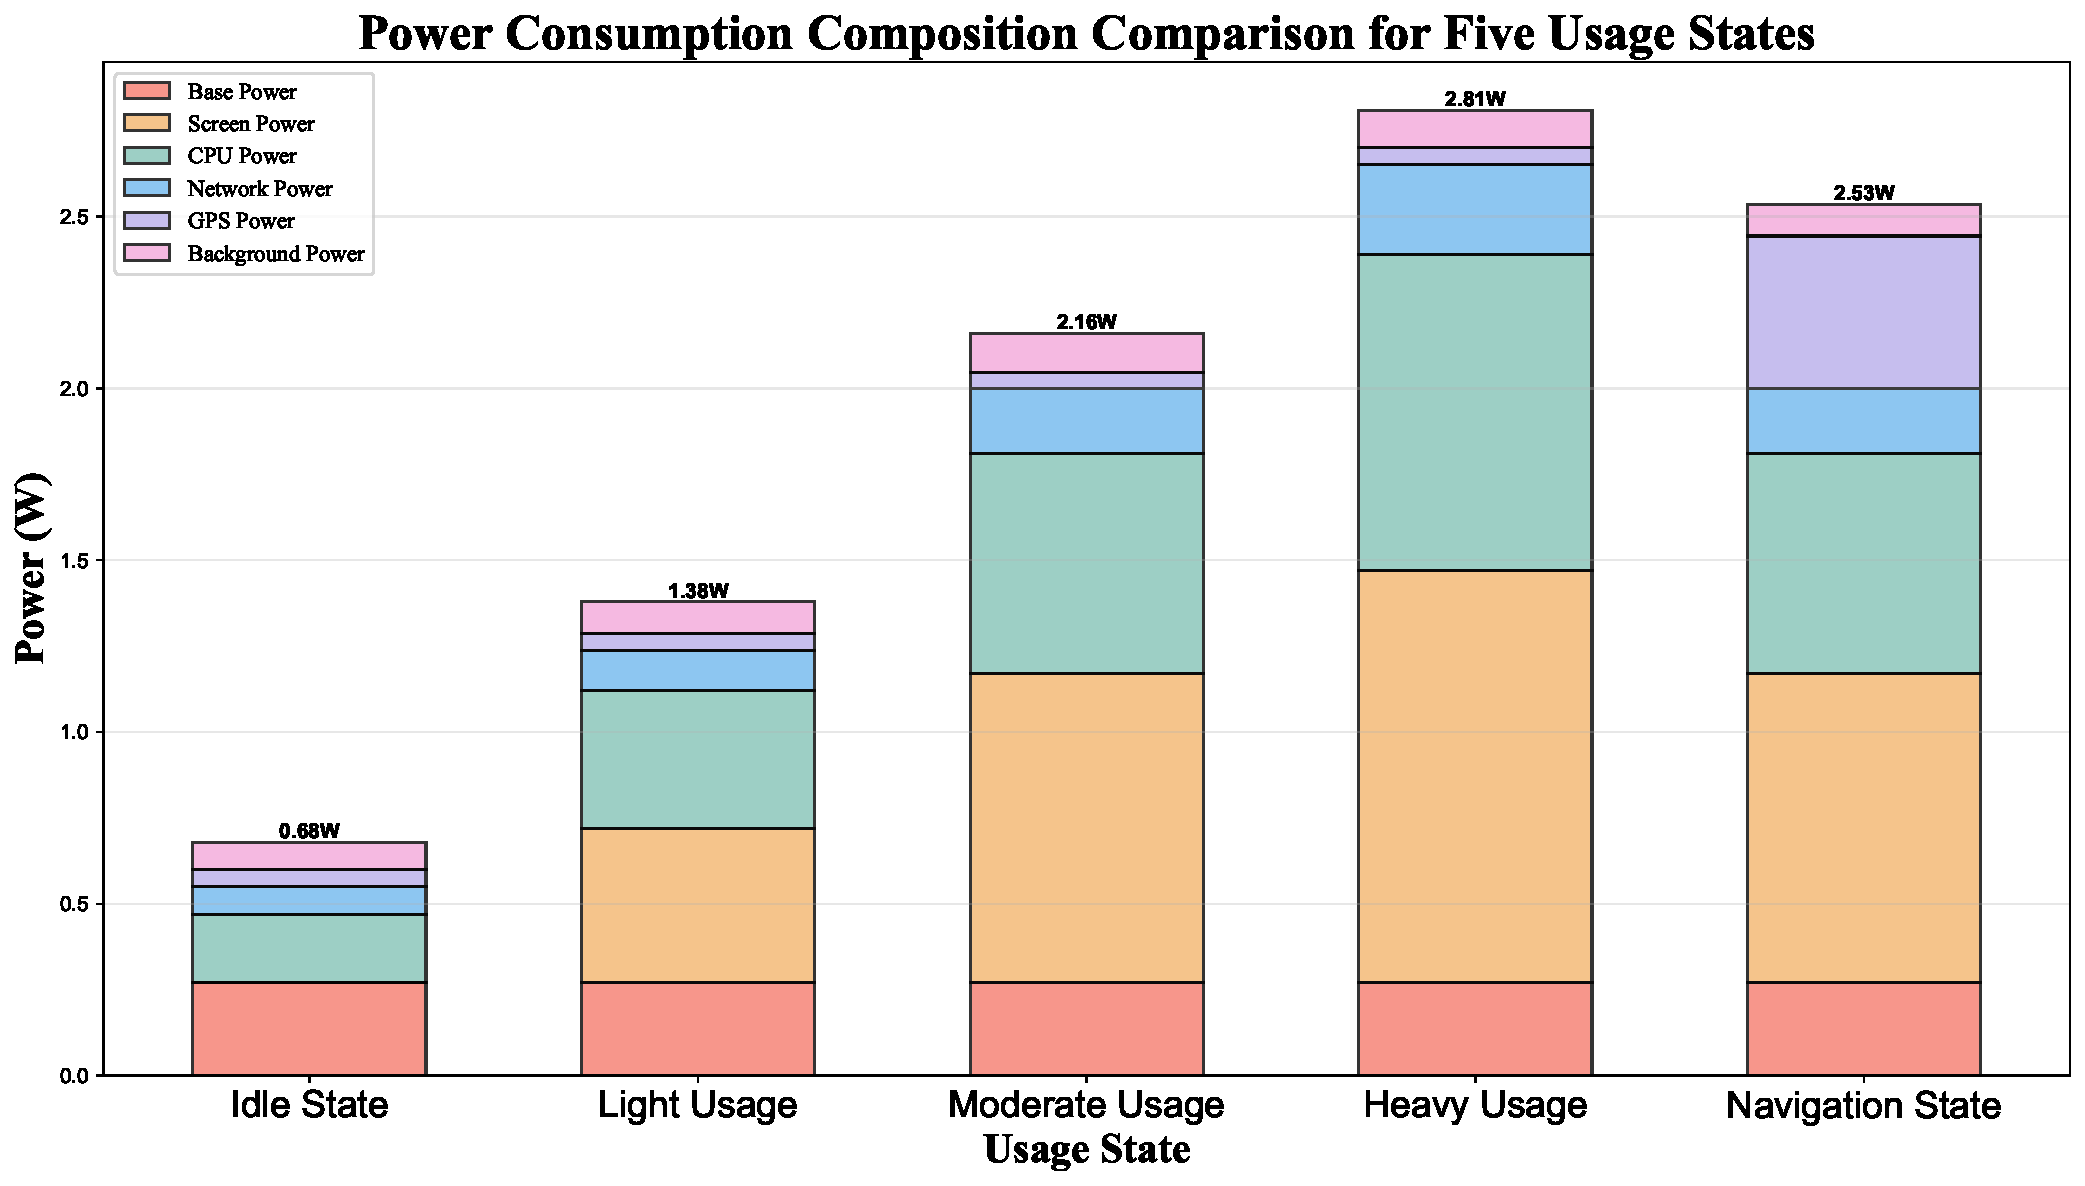
\includegraphics[width=.35\textwidth]{figures/功率.pdf}}%
		\hspace{60pt} % 自定义间距，10pt约3.5mm
		\subcaptionbox{The common value of $B(t)$\label{fig:饼状图}}
		{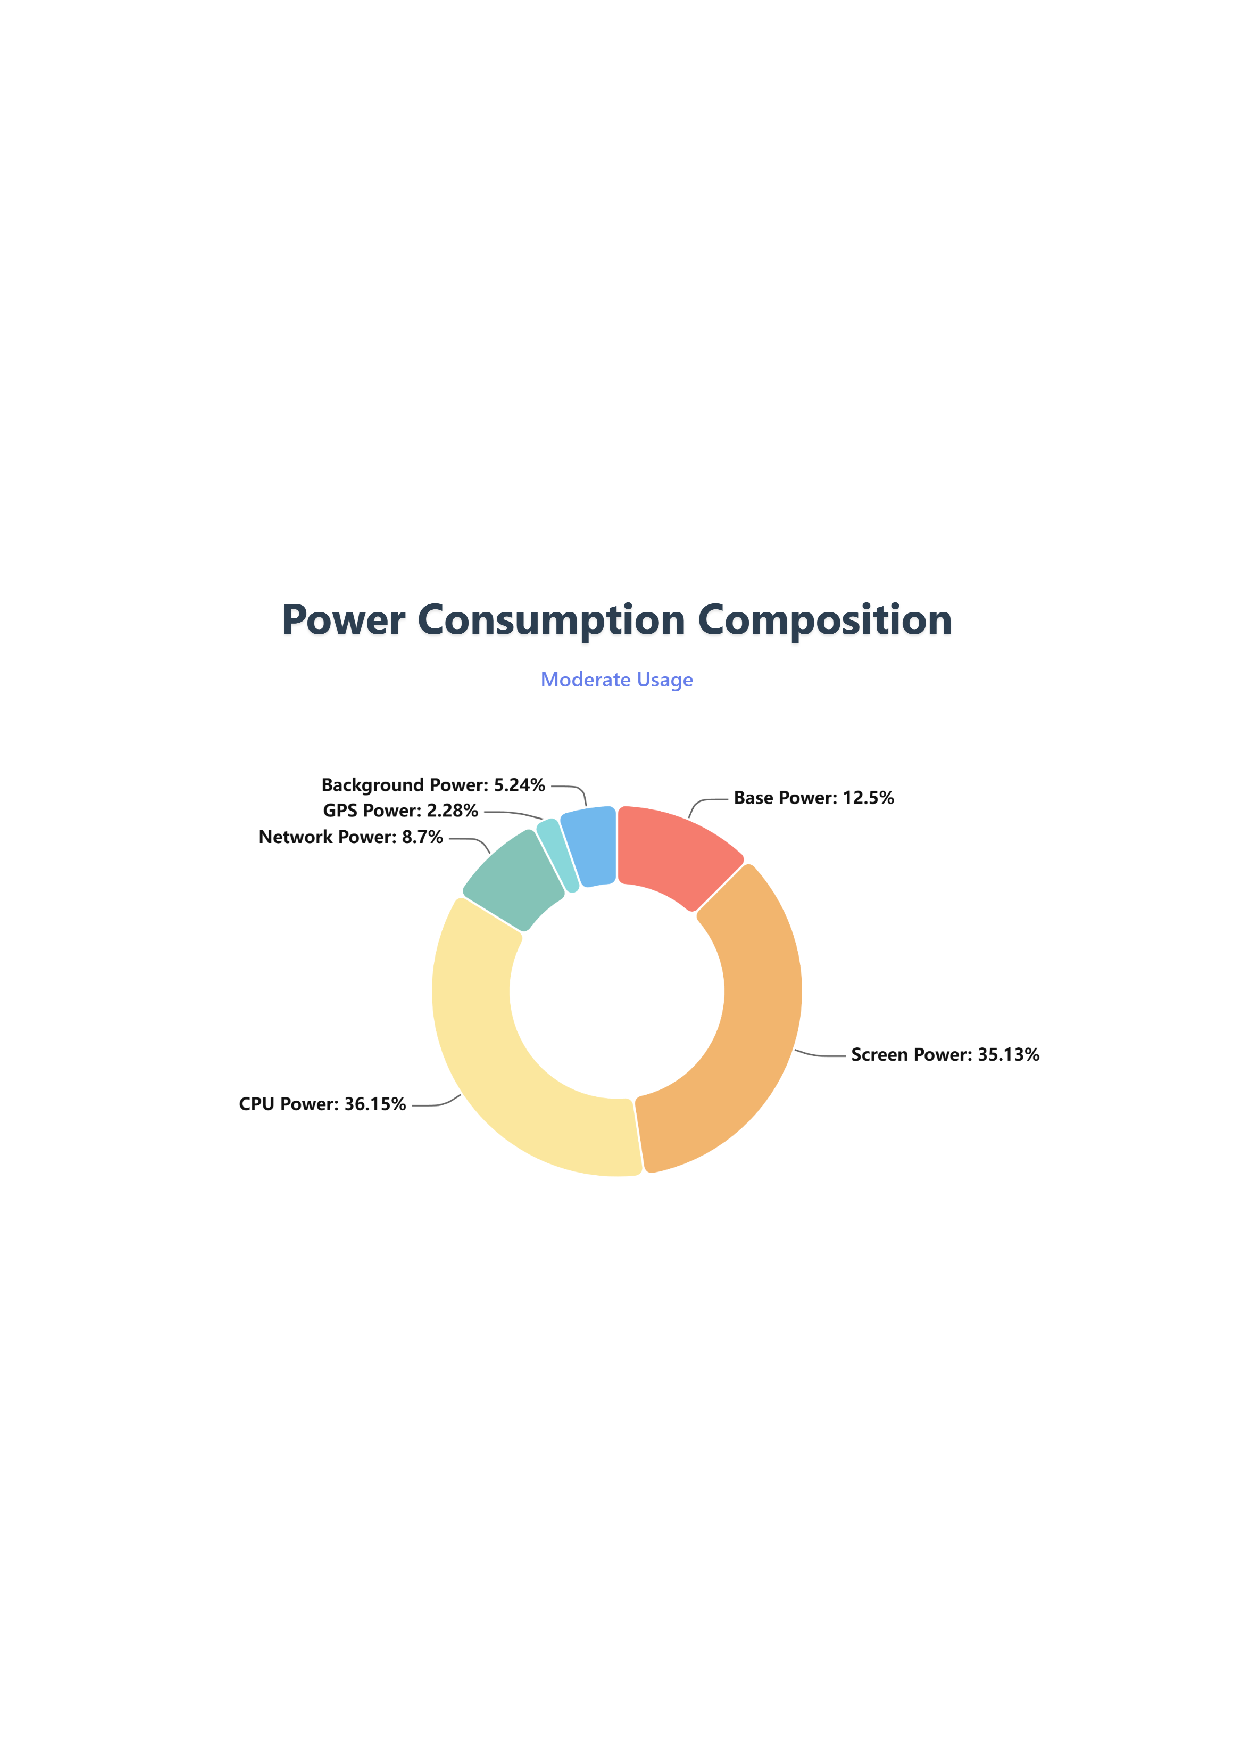
\includegraphics[width=.35\textwidth]{figures/饼状图.pdf}}
		\caption{}
		\renewcommand{\arraystretch}{1.5}
	\end{figure}
	
	为了研究各个模块对手机放电的影响，接下来我们分析了显著加快手机电池放电速度的因素。
	
	
	\subsection{显著影响因素分析}
	为识别电池续航的关键影响因素，采用控制变量法，以轻度使用模式为对照组，模拟极端但现实的使用场景，结果表明：GPS、CPU负载、屏幕亮度对电池battery life影响显著，其他模块影响较小：
	在导航模式，且其他模块的功率都处在轻度使用模式下，平均battery life减少了6小时，降幅达\textbf{40.354\%}
	在屏幕亮度最高，且其他模块的功率都处在轻度使用模式的情况下，平均battery life减少了4.85小时，降幅达\textbf{32.357\%}
	在CPU最高负载，且其他模块的功率都处在轻度使用模式下，平均battery life减少了5.9小时，降幅达\textbf{39.575\%}。
	
	
	\subsection{使用蒙特卡洛法Quantify the Uncertainty}
	
	假设变量扰动服从正态分布，采用蒙特卡洛模拟进行不确定性分析，通过标准差、变异系数（CV）、分位数区间（P5/P95）量化不确定性，变异系数是一个无量纲的统计量，用于比较不同数据集的离散程度，计算公式如下：
	\begin{equation}
		CV = \frac{\sigma}{\mu}\times100\%
		\label{eq:cv}
	\end{equation}
	
	其中，\(CV\)是变异系数，\(\sigma\)是总体标准差，\(\mu\)是总体均值。CV值越小，则相对波动性越小，数据越集中 。不确定性分析结果如表\ref{tab:控制变量}所示：
	\begin{table}[h!]
		\centering
		\renewcommand{\arraystretch}{1.5}
		\caption{在不同场景下的不确定性分析结果}
		\label{tab:控制变量}
		\begin{tabular}{lcccccc}
			\toprule
			场景 & 平均(h) & 标准差(h) & CV & P5(h) & P95(h) \\
			\midrule
			\rowcolor{pink}
			低负载-定位-10℃ & 15.9291 & 0.6611 & 0.0415 & 14.8889 & 16.9940 \\
			低负载-定位-25℃ & 14.9978 & 0.6667 & 0.0445 & 13.9795 & 16.2103 \\
			\rowcolor{pink}
			低负载-定位-40℃ & 14.1443 & 0.6233 & 0.0441 & 13.1096 & 15.2563 \\
			导航-10℃ & 10.9844 & 0.3324 & 0.0303 & 10.4562 & 11.5742 \\
			\rowcolor{pink}
			导航-25℃ & 10.3858 & 0.3037 & 0.0292 & 9.8866 & 10.8728 \\
			导航-40℃ & 9.7356 & 0.3018 & 0.0310 & 9.2585 & 10.2374 \\
			\rowcolor{pink}
			高亮度-10℃ & 10.7639 & 0.4516 & 0.0420 & 10.0645 & 11.5598 \\
			高亮度-25℃ & 10.1574 & 0.4142 & 0.0408 & 9.4838 & 10.8397 \\
			\rowcolor{pink}
			高亮度-40℃ & 9.5467 & 0.3822 & 0.0400 & 8.9356 & 10.2018 \\
			高CPU-10℃ & 9.6149 & 0.2417 & 0.0251 & 9.2173 & 10.0310 \\
			\rowcolor{pink}
			高CPU-25℃ & 9.0821 & 0.2341 & 0.0258 & 8.7323 & 9.4651 \\
			高CPU-40℃ & 8.5487 & 0.2310 & 0.0270 & 8.2051 & 8.9518 \\
			\bottomrule
		\end{tabular}
	\end{table}
	
	\newpage
	
	从表\ref{tab:控制变量}知，该模型在所有场景下的变异系数均较小，不确定性较低，模型具有较高的稳定性。相对来说在导航模式与高CPU与高网络负载的情况的平均变异系数(0.04)略高于高CPU、导航模式下的变异系数(0.03)。
	
	
	
	\section{敏感性分析与假设验证}  % 一级标题
	
	我们将通过改变假设、参数扰动、change the fluctuation in usage patterns利用预测结果的变化，来验证模型的稳定性
	
	\subsection{假设验证}
	
	我们将分别改变屏幕使用类型假设与恒温假设来验证假设的合理性
	
	\subsubsection{改变OLED屏幕假设}
	
	我们通过改变使用OLED的假设对模型对于不同屏幕类型的适配性进行验证。现改变屏幕类型为LCD，进行与上文相同的随机仿真：
	\begin{figure}[h!]
		\centering
		\renewcommand{\arraystretch}{1}
		\subcaptionbox{LCD屏的各参数同步变化的随机仿真\label{fig:同步变化的随机仿真第三问}}%
		{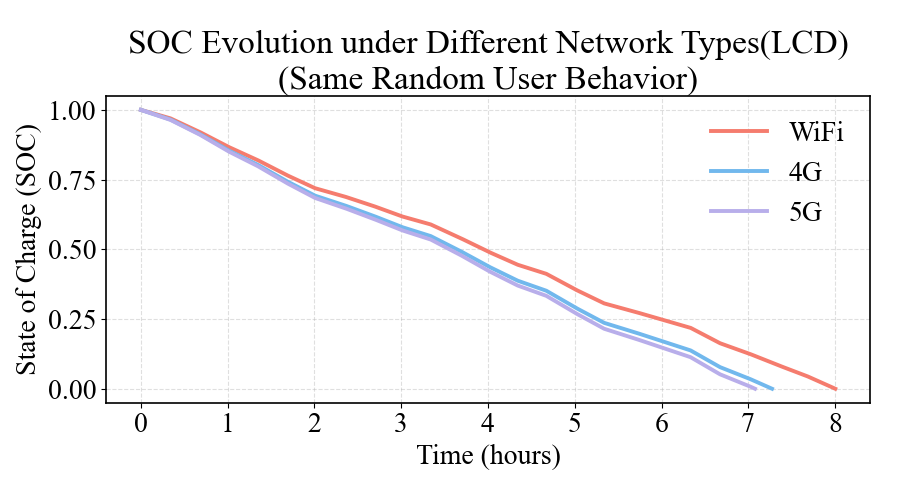
\includegraphics[width=.4\textwidth]{figures/同步变化的随机仿真第三问.png}}%
		\hspace{60pt} % 自定义间距，10pt约3.5mm
		\subcaptionbox{LCD屏的各参数独立变化的随机仿真\label{fig:独立变化的随机仿真第三问}}
		{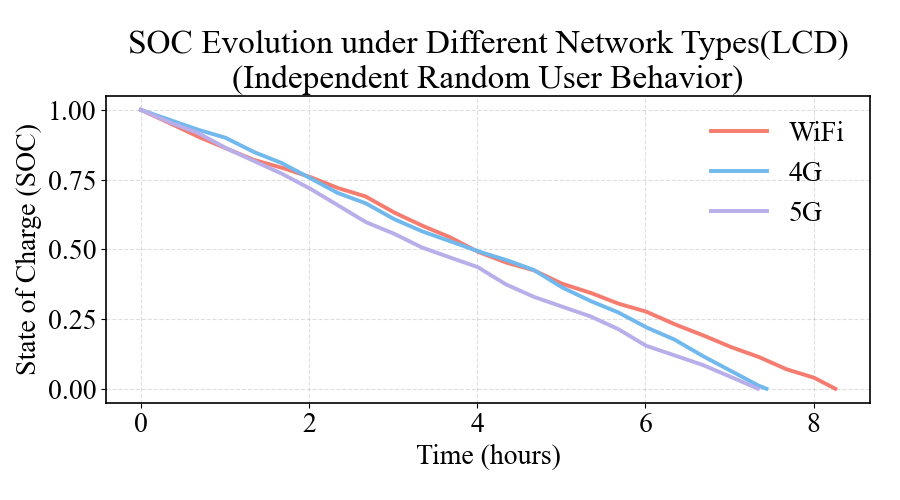
\includegraphics[width=.4\textwidth]{figures/独立变化的随机仿真第三问.png}}
		\caption{}
		\renewcommand{\arraystretch}{1.5}
	\end{figure}
	
	
	\begin{table}[h!]
		\centering
		\caption{LCD屏的各参数同步变化的随机仿真统计数据}
		\label{tab:LCD屏同步变化的随机仿真第三问}
		\renewcommand{\arraystretch}{1.5}
		\begin{tabular}{lccc}
			\toprule
			\textbf{指标} & \textbf{Wi-Fi} & \textbf{4G} & \textbf{5G} \\
			\midrule
			\rowcolor{LightGreen}
			总放电时间 (h) & 8.00 & 7.27 & 7.08 \\
			平均SOC衰减速率 (h$^{-1}$) & 0.1250 & 0.1375 & 0.1413 \\
			\rowcolor{LightGreen}
			50\% SOC放电时间 (h) & 3.95 & 3.64 & 3.56 \\
			\bottomrule
		\end{tabular}
	\end{table}
	
	\begin{table}[h!]
		\centering
		\caption{LCD屏的各参数独立变化的随机仿真统计数据}
		\label{tab:LCD屏独立变化的随机仿真第三问}
		\renewcommand{\arraystretch}{1.5}
		\begin{tabular}{lccc}
			\toprule
			\textbf{指标} & \textbf{Wi-Fi} & \textbf{4G} & \textbf{5G} \\
			\midrule
			\rowcolor{LightGreen}
			总放电时间 (h) & 8.26 & 7.44 & 7.34 \\
			平均SOC衰减速率 (h$^{-1}$) & 0.1211 & 0.1344 & 0.1363 \\
			\rowcolor{LightGreen}
			50\% SOC放电时间 (h) & 3.95 & 3.94 & 3.40 \\
			\bottomrule
		\end{tabular}
	\end{table}
	
	\newpage
	
	从相应图表得出的三种网络特点与使用OLED屏进行随机仿真得出的特点一致，表明模型对屏幕类型的适配性广泛。
	\subsubsection{改变恒温假设}
	我们引入一个微分方程来反应功率热反馈的情况：
	\begin{equation}
		C_T \frac{dT}{dt} = \eta P_{\text{total}} - h(T - T_{\text{amb}})
	\end{equation}
	
	其中，$C_T$ 为设备热容量，常见范围为$4 \sim 8\ \text{J/℃}$，$\eta$ 为功耗-热转换效率，常见范围为$0.9 \sim 1.0$，$h$ 为热传递系数，常见范围为$2\sim16\ s$。在中度使用的情况下，热反馈模型与恒温模型的随机仿真结果如图\ref{fig:考虑热反馈一致}所示：
	
	\begin{figure}[h!]
		\centering
		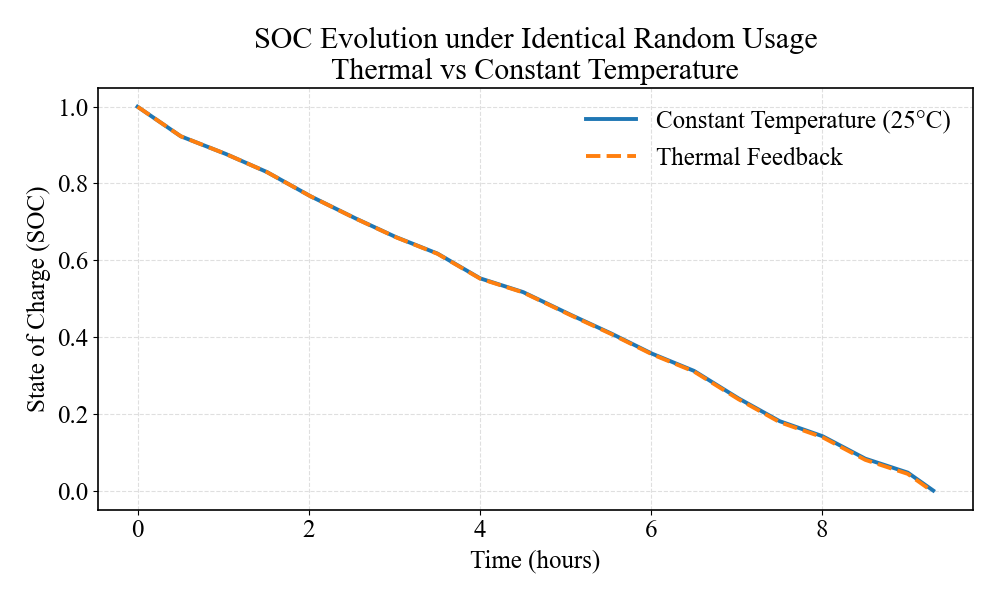
\includegraphics[width=0.5\textwidth,trim=0cm 0.4cm 0cm 0cm,clip]{figures/考虑热反馈一致.png}
		\caption{热反馈模型与恒温模型的对比结果}
		\label{fig:考虑热反馈一致}
	\end{figure}
	
	\newpage
	
	结果表明，在高负载和高环境温度条件下，热反馈会进一步缩短电池续航时间，并放大输入扰动导致的不确定性。然而，关键使用参数(CPU负载、网络活动和屏幕亮度)的敏感性排序在引入热反馈前后保持一致；恒温模型的Battery life为9.30小时，热反馈模型的battery life为9.28小时，仅变化了\textbf{0.02小时}，变化幅度仅为\textbf{0.25\%}，表明模型对假设变化具有较强鲁棒性。
	
	\subsection{敏感性分析}
	\subsubsection{Parameter values的敏感性}
	我们通过引进\textbf{Standardized RegressionCoefficient(SRC)}反映模型的参数敏感性：
	\begin{equation}
	\mathrm{SRC}_i = \beta_i \frac{\sigma_{X_i}}{\sigma_Y},
	\end{equation}
	
	其中 $\sigma_{X_i}$ 和 $\sigma_Y$ 分别为参数 $X_i$ 与输出 $Y$ 的标准差。
	SRC 的绝对值反映参数对模型输出的相对影响强度，数值越大，敏感性越强。
	
	\begin{table}[htbp]
		\centering
		\caption{各变量的SRC值}
		\renewcommand{\arraystretch}{1.1}
		\begin{tabular}{@{}cccccccccccccc@{}}
			\toprule
			变量 & $u$ & $B$ & $a_{cpu}$ & $b_{cpu}$ & $\beta$ & $r$ & $\alpha$ & $b_{wifi}$ & $a_{wifi}$ & $bg$ & $\gamma$ & $\phi_T$ & $T$ \\
			\midrule
			\rowcolor{pink}
			SRC & -0.595 & -0.492 & -0.476 & -0.311 & -0.195 & -0.136 & -0.125 & -0.116 & -0.114 & -0.070 & -0.033 & 0.001 & 0 \\
			\bottomrule
		\end{tabular}
		\label{tab:src}
	\end{table}
	
	由表\ref{tab:src}，对parameter value敏感的参数有CPU负载（$u$，SRC=-0.595）与屏幕亮度（$B$，SRC=-0.492），其中CPU负载从40\%提升至90\%可使放电时间缩短约38\%；对参数较敏感的有网络与屏幕系数和CPU系数（$a_{\text{cpu}}$，$b_{\text{cpu}}$），其10\%的误差可引起约4.8\%的放电时间预测偏差；对参数弱敏感的是温度系数（$\phi_T$，SRC=+0.001）在常温下对功耗影响可忽略，与前文分析结果一致。
	
	由于SRC基于回归分析，参数间的相关性可能导致敏感性估计偏差，因此进一步引入方差膨胀因子(Variance Inflation Factor, VIF)检验多重共线性:
	
	\begin{equation}
		\mathrm{VIF}_i = \frac{1}{1 - R_i^2}
	\end{equation}
	其中，$R_i^2$是将$X_i$对其余输入参数回归得到的决定系数。
	
	\begin{table}[htbp]
		\centering
		\caption{各变量的VIF值}
		\renewcommand{\arraystretch}{1.1}
		\begin{tabular}{@{}cccccccccccccc@{}}
			\toprule
			变量 & $\alpha$ & $\beta$ & $\gamma$ & $a_{cpu}$ & $b_{cpu}$ & $a_{wifi}$ & $b_{wifi}$ & $\phi_T$ & $B$ & $u$ & $r$ & $bg$ & $T$ \\
			\midrule
			\rowcolor{pink}
			VIF & 1.013 & 1.024 & 1.017 & 1.016 & 1.014 & 1.016 & 1.014 & 1.007 & 1.008 & 1.011 & 1.008 & 1.013 & 1.010 \\
			\bottomrule
		\end{tabular}
		\label{tab:vif}
	\end{table}
	
	计算结果显示，各主要参数的VIF值均处于常用阈值范围内，未出现显著多重共线性，表明SRC所反映的敏感性排序具有稳定性与可靠性。
	
	随后，我们同时扰动12个参数，统计的\textbf{CV值}约为5.52\%，放电时间相对波动仍保持在较低水平，模型具有较强稳定性。
	
	\begin{table}[htbp]
		\centering
		\renewcommand{\arraystretch}{1.1}
		\begin{tabular}{@{}ccccc@{}}
			\toprule
			平均放电时间 (h) & 标准差 (h) & 变异系数 (CV) & 5\%分位 (h) & 95\%分位 (h) \\
			\midrule
			\rowcolor{pink}
			12.422 & 0.685 & 0.055 & 11.372 & 13.532 \\
			\bottomrule
		\end{tabular}
		\caption{不确定性量化指标}
		\label{tab:CV}
	\end{table}
	
	\subsubsection{改变fluctuations in usage patterns}
	我们通过改变使用场景切换的频率验证模型的对鲁棒性，我们设置了2000 个行为点，间隔1分钟的基础序列，并控制所有变化组别的场景变化共享相同的基础行为序列以达到同步变化的目的，随机仿真结果如图\ref{fig:波动}所示：
	\begin{figure}[h!]
		\centering
		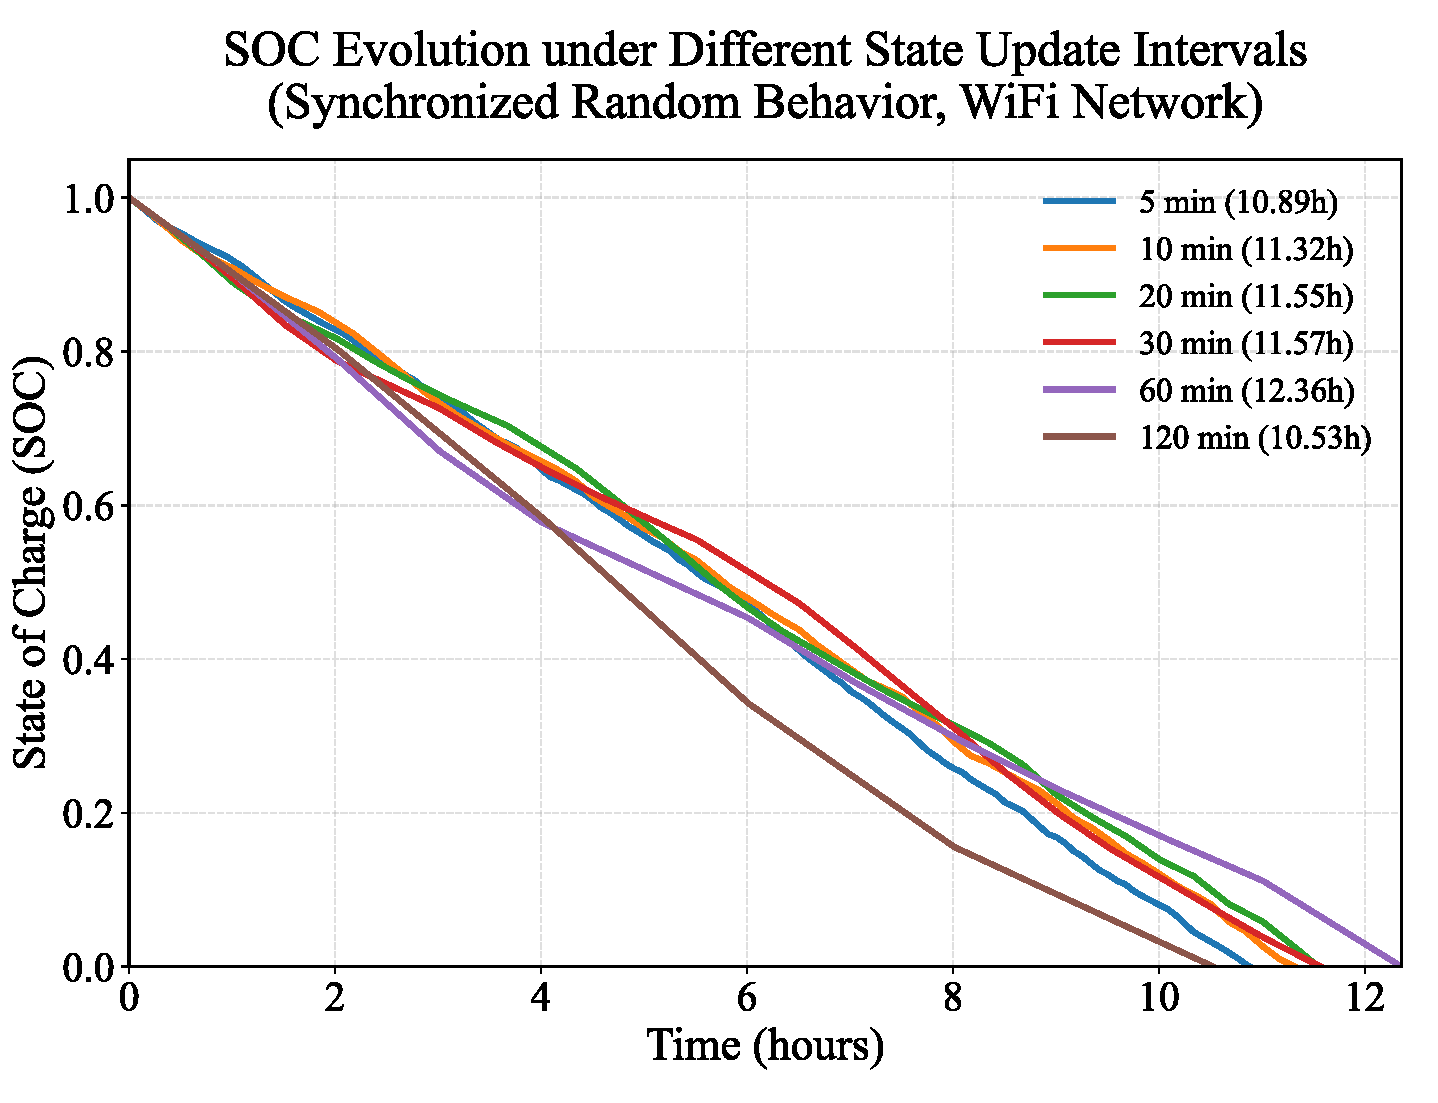
\includegraphics[width=0.5\textwidth,trim=0cm 0.4cm 0cm 0cm,clip]{figures/波动.pdf}
		\caption{不同切换频率下的随机仿真结果}
		\label{fig:波动}
	\end{figure}
	
	根据实验结果，设备的最佳更新间隔为60分钟，此时电池寿命最长可达12.36小时；而最差更新间隔为120分钟，对应电池寿命为10.53小时，两者相差1.83小时（17.4\%）。频繁更新下设备行为变化快、功耗波动大，电池效率较低；适中更新时行为变化与功耗相对稳定，电池效率较高；稀疏更新则可能导致行为变化缓慢且长期处于不利功耗状态。因此，在实际应用中建议采用约60分钟的更新间隔策略，以最大化电池寿命，相比最差情况可提升17.4\%。
	
	
	
	\section{建议}  % 一级标题
	\subsection{面向手机用户的建议}
	
	
	\begin{enumerate}[label=\arabic*.]
		\item 核心耗电模块按需开启：GPS开启续航降幅达40.354\%、CPU满负载降幅39.575\%、屏幕最高亮度降幅32.357\%，建议非导航时关闭GPS，关闭后台高负载应用，屏幕亮度调至30\%左右。
		\item 不要让手机维持在高性能模式：待机续航最长，为22.16h，重度使用仅5.36h、导航5.94h，非使用时及时切待机，减少重度/导航场景持续时长。
		\item 规避高温高负载叠加使用：40℃环境下各高耗电场景续航较10℃降低8\%-12\%，高温时避免同时使用导航、高亮度、高负载功能。
		\item 优化使用行为切换频率：每60分钟调整一次使用行为，续航可达12.36h（最优），避免超120分钟固定高功耗使用（续航仅10.53h，降幅17.4\%）。
		\item 固定场景优先用WiFi：使用配备OLED屏的手机时，WiFi续航10.66h，5G仅9,18h，建议关闭不必要的4G/5G网络。
	\end{enumerate}
	
	
	
	\subsection{面向操作系统的优化建议}
	
	
	\begin{enumerate}[label=\arabic*.]
		\item 精细化管控核心敏感参数：CPU负载（SRC=-0.595）、屏幕亮度（SRC=-0.492）为最敏感参数，实时动态调节，降低10\%参数误差可减少4.8\%续航预测偏差。
		\item 场景化智能功耗调度：自动识别5类使用场景并匹配预设功耗参数，导航场景限制非核心CPU负载，轻度使用限制屏幕亮度上限，默认60分钟场景更新间隔。
		\item 温度自适应功耗限制：设备接近40℃时，主动限制GPS、高亮度、高CPU负载功能，避免热反馈导致的续航衰减。
		\item 低不确定性续航预测：选取CV值<0.045的稳定参数区间做预测，常温下忽略温度系数（SRC=0.001）干扰，精准提示剩余续航。
		\item 网络模式智能切换：WiFi较5G续航提升12.5\%，WiFi信号稳定时自动关闭4G/5G，减少网络切换功耗激增。
	\end{enumerate}
	
	
	\subsection{关于考虑电池老化的建议}
	
	电池老化主要由日历老化与循环老化引起：日历老化表现为电池在静置状态下随时间推移的性能衰退，循环老化则源于使用过程中反复充放电造成的累积损伤。二者共同导致电池容量衰减与内阻增加。基于测量的便捷性和与用户体验的直接关联，我们选择从电池容量角度建立老化模型。
	
	\begin{equation}
		\begin{cases}
			C(t) = C_0\bigl(1 - \lambda_1 t - \lambda_2 n(t)\bigr) \\[8pt]
			C_{\text{avail}}(t) = C_{\text{eff}}(t) \left(1 - \gamma \dfrac{P_{\text{total}}(t)}{P_{\text{ref}}}\right)
		\end{cases}
	\end{equation}
	
	其中，$C(t)$ 为 $t$ 时刻电池实际可用容量；$C_0$ 为电池初始额定容量；$\lambda_1$ 为日历老化系数，反映单位时间内因静置导致的容量衰减速率（$\lambda_1\in [0.01,0.05]$ \upcite{9}）；$t$ 为电池使用时间；$\lambda_2$ 为循环老化系数，表示单次充放电循环引起的容量衰减量（$\lambda_2\in [10^{-4},10^{-3}]$ \upcite{10}）；$n(t)$ 为截至 $t$ 时刻的累计充放电循环次数。
	
	其中，$C_{\text{avail}}(t)$ 为 $t$ 时刻在当前负载下的实际可用容量；$C_{\text{eff}}(t)$ 为经日历与循环老化修正后的有效容量；$\gamma$ 为内阻-负载敏感系数，描述内阻随负载变化对可用容量的影响程度（$\gamma\in [0.05,0.2]$ \upcite{11}）；$P_{\text{total}}(t)$ 为 $t$ 时刻设备总功耗；$P_{\text{ref}}$ 为参考功率。由此得到考虑电池老化的电量演化微分方程：
	
	\begin{equation}
		\frac{d \left(\text{SOC}(t)\right)}{dt} = - \frac{P_{\text{total}}(t)}{C_0 \cdot \bigl(1 - \lambda_1 t - \lambda_2 n(t)\bigr) \cdot V \, \Phi(T) \cdot \left(1 - \gamma \frac{P_{\text{total}}(t)}{P_{\text{ref}}}\right)}
	\end{equation}
	
	考虑电池老化对续航的影响，我们建议用户在长期闲置时将电量保持在50\%--80\%并每三个月检查补电；日常使用尽量维持电量在20\%--80\%之间，避免深度放电与长期满电；若电池出现续航锐减、异常发热或外形膨胀等问题，应及时检测或更换。同时，建议厂商内置电池健康度监测功能，在健康度降至80\%时提醒用户更换电池或设备。
	
	
	\subsection{模型延伸：跨设备适配}
	
	最后，将所建模型推广至其他便携式智能设备，本文选取智能手环作为代表性分析对象。已有研究表明，智能手环的电池寿命变化同样受到用户使用行为的显著影响\upcite{12}。与智能手机相比，智能手环在硬件结构与使用方式上具有电池容量更小、计算负载更低以及通信方式以低功耗蓝牙为主等特点。因此，在不改变模型整体结构的前提下，仅需对关键参数进行合理重标定，即可实现模型在该类设备上的适配。
	
	\begin{figure}[h!]
		\centering
		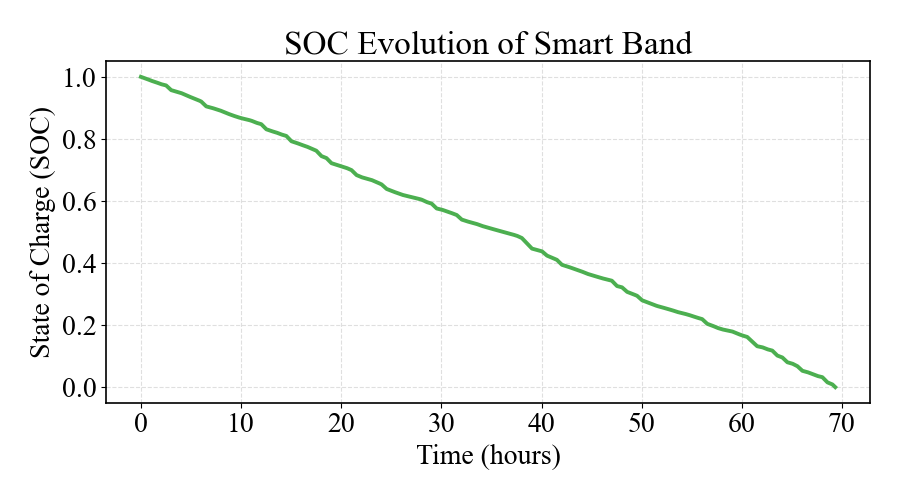
\includegraphics[width=0.5\textwidth,trim=0cm 0.4cm 0cm 0cm,clip]{figures/手环.png}
		\caption{模型在智能手环上的应用}
		\label{fig:手环}
	\end{figure}
	
	在随机仿真过程中，智能手环的电量变化趋势与前文模型中的演化规律保持一致，表明模型在不同设备场景下具有良好的稳定性。基于调整后的参数进行仿真，得到智能手环的电池续航时间约为 69.3 小时，该结果与现有研究结论及实际使用情况较为接近，具有较好的合理性与现实意义。由此可见，本文所构建的功耗模型具备良好的可推广性，能够通过参数调整有效应用于多种便携式智能设备。
	
	
	
	
	\section{Model Evaluation}  % 一级标题
	\subsection{Strengths}
	
	\begin{itemize}
		\item \textbf{模型结构可靠性：}本文以连续时间SOC状态微分方程为框架，以系统总功耗作为SOC动态变化的驱动项，无需深入涉及电池内部复杂工作原理，既简化了模型复杂度，又保障了模型良好的结构可靠性与物理合理性。
		\item \textbf{参数选取科学性：}模型所涉及的各项功耗系数、电池老化系数等关键参数，均严格参照相关公开学术文献及权威测量报告中的合理取值范围确定，确保参数选取的科学性，与实际应用场景高度贴合。
		\item \textbf{数据应用合理性：}本文所采用的数据主要用于校验功耗的合理性及参数取值的准确性，而不用于SOC时间序列进行拟合或回归分析。
		\item \textbf{模型泛化性：}模型可推广应用于手环、平板电脑、笔记本电脑等多种便携式电子设备。通过针对性调整电池容量、系统功耗基准值、温度修正系数等核心参数，即可适配不同设备的硬件特性与使用场景。
	\end{itemize}
	
	\subsection{Weaknesses}
	
	\begin{itemize}
		\item 模型验证主要依赖于学术文献、行业报告及公开测试数据等公开数据集，缺乏大规模、多维度的真实场景实测数据进一步验证。
		\item 模型虽已采用随机仿真与场景参数化的方法覆盖了各类核心差异，但仍难以精细化捕捉不同App的后台行为异质性与硬件型号特异性等方面的差异，同时也无法精准模拟真实用户的碎片化使用行为。
	\end{itemize}
	
	
	\subsection{Improvement}
	
	\begin{itemize}
		\item \textbf{实测数据验证：}联合相关实验室或招募不同使用习惯的用户，开展多设备、多环境、长周期的实测实验，补充真实场景实测数据，强化模型验证的全面性与可靠性。
		\item \textbf{行为驱动建模与设备自适应：}构建硬件型号参数库并引入参数自适应调整机制，实现模型对多类电子设备的精准适配。同时优化用户行为模拟方式，还原用户碎片化使用行为的随机性与复杂性。
	\end{itemize}
	
	
	
	
	
	\newpage
	\phantomsection  % 创建锚点
	\addcontentsline{toc}{section}{References}
	\begin{thebibliography}{99}%宽度9
		\bibitem{1} CARROLL A, HEISER G. An Analysis of Power Consumption in a Smartphone[C]//Proc. 2010 USENIX conf., USENIX Assoc. 2010.
		\bibitem{2} Dash, P., \& Hu, Y. C. (2021). How much battery does dark mode save? An accurate OLED display power profiler for modern smartphones. In \textit{Proceedings of the 19th Annual International Conference on Mobile Systems, Applications, and Services} (pp. 1–13). ACM. https://doi.org/10.1145/3458864.3467682
		\bibitem{3} DONG M, CHOI Y S K, ZHONG L. Power modeling of graphical user interfaces on OLED displays[C/OL]//2009 46th ACM/IEEE Design Automation Conference. 2009: 652-657[2026-01-31]. https://ieeexplore.ieee.org/document/5227097.
		\bibitem{4} CHOI Y, HA R, CHA H. Fully automated OLED display power modeling for mobile devices[J/OL]. Pervasive and Mobile Computing, 2018, 50: 41-55. DOI:10.1016/j.pmcj.2018.07.006.
		\bibitem{5} R. Cheng, J. Lu, H. Jiang, et al., "Research on energy consumption model of intelligent mobile terminals," *Computer Technology and Development*, vol. 27, no. 12, pp. 128-132, 138, Dec. 2017.
		\bibitem{6} Gupta, A., Heidari, A., Kalipattapu, A., et al. (2024). 3 W’s of smartphone power consumption: Who, Where and How much is draining my battery? In \textit{Proceedings of the 30th Annual International Conference on Mobile Computing and Networking} (pp. 2248–2250). Association for Computing Machinery. https://doi.org/10.1145/3636534.3695905
		\bibitem{7}Kim J H, Lee S J, Kim Y J. Temperature-dependent performance of smartphone batteries[J]. IEEE Transactions on Consumer Electronics, 2015, 61(3): 292-298.
		\bibitem{8}Huang, X. H., \& Hu, Z. H. (2012). A brief analysis of the Runge-Kutta method. *Heilongjiang Science and Technology Information*, (23), 28.
		\bibitem{9}Ali, H., Beltran, H., Lindsey, N. J., \& Pecht, M. (2023). Assessment of the calendar aging of lithium-ion batteries for a long-term—Space missions. Frontiers in Energy Research, 11. https://doi.org/10.3389/fenrg.2023.1108269
		\bibitem{10}Gantenbein, S., Schönleber, M., Weiss, M., \& Ivers-Tiffée, E. (2019). Capacity Fade in Lithium-Ion Batteries and Cyclic Aging over Various State-of-Charge Ranges. Sustainability, 11(23), 6697. https://doi.org/10.3390/su11236697
		\bibitem{11}Li, W., Zhang, H., van Vlijmen, B., Dechent, P., \& Sauer, D. U. (2021). Forecasting battery capacity and power degradation with multi-task learning [Preprint]. arXiv. https://arxiv.org/abs/2111.14937
		\bibitem{12}Sunder, R., Lilhore, U. K., Rai, A. K., et al. (2025). SmartAPM framework for adaptive power management in wearable devices using deep reinforcement learning. *Scientific Reports*, *15*, 6911. https://doi.org/10.1038/s41598-025-89709-3
	\end{thebibliography}
	
	%%%%%%%%%%%%%%%%%%%%%%% 正文结束 %%%%%%%%%%%%%%%%%%%%%%%
	
	\newpage
	\section*{\centering Report on Use of AI Tools}
	
	\subsection*{1. OpenAI ChatGPT (Feb 2, 2026 version, GPT-5.2)}
	\begin{itemize}
		\item \textbf{Query}: Could you please provide relevant literature and links on mobile phone power consumption, so that we can examine the parameters of our established model?
		\item \textbf{Output}: Here are some important academic papers on smartphone power (energy) modeling, analysis, and optimization, along with accessible links, which are suitable for building, validating, or comparing parameters of power models:
		\begin{enumerate}[label=(\arabic*)]
			\item \textit{Modeling of Smartphones Power Using Neural Networks} — Uses neural networks to build a smartphone power prediction model, analyzing the relationship between user behavior and power consumption.
			\item \textit{The Influence of Temperature on the Capacity of Lithium Ion Batteries with Different Anodes} — This study can be used to analyze the impact of temperature on smartphone battery performance, with relevant parameters available.
			\item \textit{An Analysis of Power Consumption in a Smartphone} — This seminal research provides a comprehensive analysis of various factors affecting power consumption in smartphones, which can be referenced.
		\end{enumerate}
	\end{itemize}
	
	\subsection*{2. OpenAI ChatGPT (Feb 2, 2026 version, GPT-5.2)}
	\begin{itemize}
		\item \textbf{Query}: What are the key concepts related to the Standardized Regression Coefficient (SRC) and the Coefficient of Variation (CV)?
		\item \textbf{Output}: Both SRC and CV are tools that use standardization to eliminate differences in units, but they serve different purposes: SRC is used in regression analysis to fairly compare the influence of different variables on an outcome, while CV is used in descriptive statistics to compare the variability (or stability) between different datasets. In simple terms, SRC compares the impact of variables, whereas CV compares the stability of the data itself.
	\end{itemize}
	
	\subsection*{3. OpenAI ChatGPT (Feb 2, 2026 version, GPT-5.2)}
	\begin{itemize}
		\item \textbf{Query}: What is the technical principle of stochastic simulation?
		\item \textbf{Output}: The fundamental principle of random state switching simulation is to abstract the system into several discrete states. It assumes that the system remains in a given state for a random duration and then switches to another state according to specified transition probabilities. Both the dwell time and state transitions are determined by random variables, typically implemented by generating uniform random numbers and sampling from probability distributions. By repeatedly performing the process of “randomly sampling dwell time—updating system time—selecting the next state based on transition probabilities,” a stochastic trajectory of the system state over time can be obtained. This allows for the analysis of statistical properties and long-term behavior after multiple simulation runs.
	\end{itemize}
	
	\subsection*{4. GitHub Copilot (Grok Code Fast 1 version)}
	\begin{itemize}
		\item \textbf{Query}: Please help me check for code defects and complete the code, without altering the original functionality of the code.
		\item \textbf{Output}: Auto‑completions for code used in preparing our models.
	\end{itemize}
	
	\subsection*{5. ByteDance Doubao (Aug 20, 2024 version, Seed Large Model)}
	\begin{itemize}
		\item \textbf{Application}: We employed it to conduct translation, language refinement, and the modification and tuning of LaTeX code.
	\end{itemize}
	
\end{document}  % 文档结束
%%%%%%%%%%%%%%%%%%%%%%%%%%%%%%%%%%%%%%%%%%%%%%%%%%%%%%%